\documentclass[12pt,openany]{book}

\usepackage[utf8]{inputenc}
\usepackage[T1]{fontenc}
\usepackage{microtype}
\usepackage{amsmath,amssymb}
\usepackage{geometry}
\usepackage[colorlinks=true, linkcolor=black, citecolor=black, urlcolor=blue]{hyperref}
\usepackage{setspace}
\usepackage{tikz}
\usetikzlibrary{shapes,positioning,calc,decorations.pathreplacing}
\usepackage{titlesec}
\usepackage{fancyhdr}
\usepackage[most]{tcolorbox}
\usepackage{graphicx}

\geometry{inner=1.2in, outer=1in, top=1in, bottom=1in}
\onehalfspacing
\emergencystretch=1em

% --- Custom chapter heading style ---
\titleformat{\chapter}[display]
  {\normalfont\huge\bfseries}
  {\titlerule[1pt]\vspace{4pt}\Large\chaptertitlename\ \thechapter}
  {0pt}
  {\titlerule[1pt]\vspace{8pt}\Huge}
\titlespacing*{\chapter}{0pt}{-20pt}{30pt}

% --- Running headers/footers ---
\pagestyle{fancy}
\setlength{\headheight}{27.11469pt}
\addtolength{\topmargin}{-15.11469pt}
\fancyhf{}
\fancyhead[LE]{\slshape\leftmark}
\fancyhead[RO]{\slshape\rightmark}
\fancyfoot[C]{\thepage}

\renewcommand{\headrulewidth}{0.4pt}
\fancypagestyle{plain}{%
  \fancyhf{}%
  \fancyfoot[C]{\thepage}% 
  \renewcommand{\headrulewidth}{0pt}%
}

% --- Boxed environments ---
\newtcolorbox{definition}[1][]{%
  colback=blue!5, colframe=blue!60!black,
  fonttitle=\bfseries, title={#1},
  breakable, enhanced,
  before upper={\parindent15pt},
  boxrule=1pt, arc=3pt
}

\newtcolorbox{keyinsight}[1][]{%
  colback=green!5, colframe=green!50!black,
  fonttitle=\bfseries, title={#1},
  breakable, enhanced,
  before upper={\parindent15pt},
  boxrule=1pt, arc=3pt
}

\newtcolorbox{historicalsource}[1][]{%
  colback=orange!5, colframe=orange!70!black,
  fonttitle=\bfseries, title={#1},
  breakable, enhanced,
  before upper={\parindent15pt},
  boxrule=1pt, arc=3pt
}

\title{The Mathematics of Oppression:\\A Set-Theoretic Framework for Analyzing Systems of Domination}
\author{Emmanuel Theodore}
\date{}

\begin{document}

% --- Half-title page ---
\thispagestyle{empty}
\vspace*{\fill}
\begin{center}
{\Huge\bfseries The Mathematics of Oppression}
\end{center}
\vspace*{\fill}
\cleardoublepage

% --- Full title page ---
\maketitle

% --- Front matter ---
\frontmatter
\tableofcontents
\listoffigures

\chapter*{Preface}
\addcontentsline{toc}{chapter}{Preface}

This book develops a formal mathematical framework for analyzing systems of oppression using set theory, discrete mathematics, and historical analysis. The framework identifies four architectural components common to all oppressive systems: (1) asymmetric autonomy restriction between In-groups and Out-groups, (2) selective empathy that validates In-group suffering while dismissing Out-group harm, (3) ideological justification through spurious claims, and (4) resistance to structural critique. The system is operationalized through a five-tier hierarchy: the true Elite ($E$), the Puppet Class ($P_{\text{uppet}}$), the Enforcement Class ($F_{\text{enforce}}$), the Buffer Class ($I_{\text{buffer}}$), and the racialized Out-group ($O_{\text{racialized}}$). Through detailed analysis of American racism---tracing the algorithm of Elite extraction from Portuguese racialization through Bacon's Rebellion, the invention of whiteness, the 13th Amendment loophole, redlining, the War on Drugs, and the present-day cannibalization of the In-group---I demonstrate that the Out-group targeted by systemic oppression \textit{expands} over time, progressively encompassing groups once part of the In-group. This expansion reveals that oppressive systems serve not the nominal In-group but an Elite class ($E \subset I$) that uses division to prevent solidarity. The architecture of this system---a Predatory Min-Max Function that maximizes extraction while minimizing class resistance---operates through recognizable, formalizable patterns that can be identified and resisted.

% --- Main matter ---
\mainmatter

\chapter{Redefining Racism}

This paper proposes a mathematical framework for understanding systems of oppression---social arrangements that systematically disadvantage a racialized Out-group ($O_{\text{racialized}}$) while advantaging an In-group ($I$), though the true beneficiaries are a small Elite class ($E \subset I$) that architects the system. The framework reveals a five-tier operational hierarchy: the Elite ($E$) extracts value, the Puppet Class ($P_{\text{uppet}}$) writes the laws, the Enforcement Class ($F_{\text{enforce}}$) physically actuates the extraction, the Buffer Class ($I_{\text{buffer}}$) receives psychological wages in lieu of material benefit, and $O_{\text{racialized}}$ bears the compounding burden of policy after policy. Traditional analyses of oppression often focus on individual prejudice or specific policy outcomes. However, such approaches fail to capture the \textit{structural} dimensions of oppression: the recurring patterns, the self-reinforcing mechanisms, and the remarkable consistency of design across different systems and scales.

The central thesis of this paper is that domination has one architecture. The same extraction algorithm is statistically self-similar across every scale and every domain. The five-tier hierarchy and the Predatory Min-Max Function are the invariant geometry of that architecture. Every formal language deployed in this paper---electrodynamics, software engineering, set theory---describes the identical structure. The algorithm expands the Out-group over time, progressively absorbing groups once protected by the In-group boundary, because the system serves an Elite class that manufactures division to prevent solidarity. This architecture consists of:
\begin{enumerate}
    \item \textbf{Asymmetric autonomy restriction}: Policies and norms that constrain the Out-group's freedom while preserving the In-group's
    \item \textbf{Selective empathy}: Validation of In-group suffering while dismissing or pathologizing Out-group harm
    \item \textbf{Ideological justification}: Narratives that naturalize the asymmetry through spurious claims
    \item \textbf{Resistance to structural critique}: Mechanisms that deflect analysis from the system to individual behavior
\end{enumerate}

To develop and validate this framework, I examine \textbf{racism} as the primary case study---specifically, the American system of racial oppression from its colonial origins to the present. Racism provides an ideal test case because of its extensive historical documentation, its clear policy mechanisms, and its ongoing relevance. Through set-theoretic analysis, I demonstrate that racism exhibits all four architectural components and, crucially, that $O_{\text{racialized}}$ has \textit{expanded} over time rather than contracted.

This expansion reveals a deeper truth: the system does not ultimately serve the racial In-group but rather the Elite class ($E \subset I$) that uses racial division to prevent cross-group solidarity. The ``wages of whiteness'' \cite{roediger, dubois}---psychological compensation offered to the buffer class $I \setminus E$---substitute for material advancement while $E$ extracts value from both groups.

The architecture of this system---which I formalize as a Predatory Min-Max Function optimizing Elite extraction against class resistance---operates through recognizable patterns that can be formalized, identified, and resisted across contexts.

\textbf{A critical methodological note}: Comparing the \textit{architecture} of different oppressive systems does not equate their \textit{phenomenology}. This paper analyzes design principles---how asymmetry is created, justified, and maintained---not magnitudes of suffering. Recognizing shared structure illuminates how systems of domination reproduce themselves; it does not diminish the unique gravity of any particular manifestation.

\section{Racism as Primary Example}

\textbf{The Problem with Traditional Definitions}

Traditional definitions of racism reveal a troubling pattern: they relegate the systemic dimension to secondary or tertiary status, often buried as the third or fourth definition in dictionaries---the ``cliff notes'' version that few people encounter or use. Consider typical definitional hierarchies:

\begin{enumerate}
    \item \textbf{Primary definition}: Individual prejudice or discrimination based on race
    \item \textbf{Secondary definition}: Belief in racial superiority
    \item \textbf{Tertiary definition} (if present at all): Systemic or institutional discrimination
\end{enumerate}

This ordering is not merely unfortunate---it is \textbf{fundamentally backwards}. By centering individual prejudice, these definitions obscure the cardinal reality: \textit{the systemic element is the primary operation}. The interpersonal manifestations---individual prejudice, discriminatory actions, racial animus---are \textit{downstream products} created to maintain the systemic structure, not the cause of it.

\textbf{Reversing the Causal Arrow}

The conventional framing suggests this causal relationship:
\[
\text{Individual Prejudice} \rightarrow \text{Discriminatory Actions} \rightarrow \text{Systemic Outcomes}
\]

This implies that if we eliminate individual prejudice, systemic racism will disappear. But history reveals the opposite causal structure:
\[
\text{Elite Economic Interests} \rightarrow \text{Systemic Racialization} \rightarrow \text{Interpersonal Prejudice}
\]

As demonstrated in Chapter 2, interpersonal racism---the attitudes, beliefs, and prejudices held by individuals---\textit{was deliberately created to justify and maintain the systemic structure}. Zurara's racialization of Africans as subhuman was not a spontaneous expression of Portuguese prejudice; it was commissioned work designed to justify a system of unlimited exploitation \cite{zurara, biewen}. The interpersonal followed the systemic, not vice versa (see Figure~\ref{fig:causal_reversal}).

\begin{figure}[htbp]
\centering
\begin{tikzpicture}[
    box/.style={draw, thick, rounded corners=3pt, minimum height=0.9cm, minimum width=2.6cm, align=center, font=\small},
    arr/.style={->, thick, >=stealth},
    scale=0.95
]
    % --- Conventional (incorrect) row ---
    \node[font=\small\bfseries, red!60] at (-5.8,1.5) {Conventional};
    \node[font=\small\bfseries, red!60] at (-5.8,1.0) {(incorrect)};
    \node[box, fill=red!10, draw=red!40] (a1) at (-2.5,1.25) {Individual\\Prejudice};
    \node[box, fill=red!10, draw=red!40] (a2) at (2,1.25) {Discriminatory\\Actions};
    \node[box, fill=red!10, draw=red!40] (a3) at (6.5,1.25) {Systemic\\Outcomes};
    \draw[arr, red!40] (a1) -- (a2);
    \draw[arr, red!40] (a2) -- (a3);
    % Strike-through
    \draw[very thick, red!50] (-4.5,1.25) -- (8.5,1.25);

    % --- Reversal arrow ---
    \draw[arr, very thick, black!70, double] (1.5,0.3) -- (1.5,-0.5);
    \node[font=\footnotesize\bfseries, black!70] at (3.2,-0.1) {Causal reversal};

    % --- Correct row ---
    \node[font=\small\bfseries, green!50!black] at (-5.8,-1.25) {Actual};
    \node[font=\small\bfseries, green!50!black] at (-5.8,-1.75) {(historical)};
    \node[box, fill=green!15, draw=green!50!black] (b1) at (-2.5,-1.5) {Elite Economic\\Interests};
    \node[box, fill=green!15, draw=green!50!black] (b2) at (2,-1.5) {Systemic\\Racialization};
    \node[box, fill=green!15, draw=green!50!black] (b3) at (6.5,-1.5) {Interpersonal\\Prejudice};
    \draw[arr, green!50!black, very thick] (b1) -- (b2);
    \draw[arr, green!50!black, very thick] (b2) -- (b3);
\end{tikzpicture}
\caption{\textbf{The Causal Reversal.} The conventional framing (top, struck through) assumes individual prejudice produces systemic outcomes. The historical evidence (bottom) reveals the opposite: Elite economic interests created systemic racialization, which then cultivated interpersonal prejudice to maintain the structure.}
\label{fig:causal_reversal}
\end{figure}

\textbf{The Linguistic Evidence}

Moreover, traditional definitions overlook a fundamental linguistic aspect: the suffix ``-ism'' in ``racism'' already denotes a \textit{system}. We recognize this in other contexts:
\begin{itemize}
    \item \textbf{Capitalism}: A \textit{system} of economic organization, not just individual acts of trade
    \item \textbf{Feudalism}: A \textit{system} of social hierarchy, not just individual lord-serf relationships
    \item \textbf{Colonialism}: A \textit{system} of territorial exploitation, not just individual acts of conquest
\end{itemize}

Yet with racism, we persistently treat it as a collection of individual attitudes rather than recognizing the systemic nature embedded in the very structure of the word. This is not accidental---it serves to deflect attention from the structural mechanisms that create and perpetuate racial inequality.

\textbf{The Critical Distinction: Racism is Not Prejudice}

This analysis reveals a fundamental conceptual error in conflating racism with prejudice or bias. The distinction is not one of degree but of \textit{kind}:

\begin{quote}
\textbf{Prejudice or bias}: Individual attitudes, stereotypes, or discriminatory behaviors based on group membership. These are interpersonal phenomena that can exist in any direction and between any groups.

\textbf{Racism}: A \textit{system of oppression} that weaponizes prejudice and bias into structural mechanisms of exploitation and control. Racism takes individual prejudice and transforms it through institutionalization into a self-perpetuating apparatus that serves Elite economic interests.
\end{quote}

\textbf{Without the systemic element, there is no racism---there is only prejudice.} The system is not an optional feature or a more severe manifestation; it is the \textit{defining characteristic} that distinguishes racism from generic bias. Consider:

\begin{itemize}
    \item A person holding negative stereotypes about another group = \textbf{prejudice}
    \item A system that codifies those stereotypes into law, policy, and institutional practice to extract labor and prevent solidarity = \textbf{racism}
\end{itemize}

Racism is the process of taking interpersonal prejudice and bias---which exist across all human societies---and \textbf{weaponizing them} into a system that:
\begin{enumerate}
    \item \textbf{Institutionalizes} prejudice through policy ($P$)
    \item \textbf{Concentrates} harm at the intersection $O_{\text{racialized}} \cap P$
    \item \textbf{Naturalizes} the resulting disparities through ideology
    \item \textbf{Compounds} disadvantage over time through the mechanisms described in Chapter~3
    \item \textbf{Serves} Elite economic interests by preventing working-class solidarity
\end{enumerate}

This distinction has profound implications. An individual can hold prejudices without participating in racism if those prejudices are not institutionalized into systems of power. Conversely, an individual can participate in and benefit from racist systems even while holding no conscious prejudice---because racism operates \textit{systemically}, through policies and structures, not merely through individual attitudes.

The conflation of racism with prejudice is not merely imprecise---it is \textbf{functionally useful to the system}. By treating them as synonymous, we:
\begin{itemize}
    \item Suggest that eliminating individual prejudice eliminates racism
    \item Enable individuals to disavow racism by disavowing prejudice
    \item Obscure the structural mechanisms that create and maintain racial hierarchy
    \item Deflect attention from the Elite class that benefits from racial division
    \item Make structural analysis seem like an overreaction to individual attitudes
\end{itemize}

The system is \textit{the point}. Racism is fundamentally and irreducibly systemic. Without the system, we're discussing prejudice, bias, or discrimination---real phenomena, but categorically different from racism as a system of oppression.

\textbf{Why the Misdirection Matters}

Centering individual prejudice as the primary definition of racism accomplishes several functions that protect the systemic structure:

\begin{enumerate}
    \item \textbf{Individualizes responsibility}: If racism is primarily individual prejudice, then solutions focus on changing hearts and minds rather than dismantling structures.
    
    \item \textbf{Obscures Elite benefits}: Individual-focused definitions hide the fact that racism serves Elite economic interests by preventing working-class solidarity.
    
    \item \textbf{Enables plausible deniability}: Individuals can claim ``I'm not racist'' (meaning ``I don't hold personal prejudice'') while participating in and benefiting from racist systems.
    
    \item \textbf{Makes structural critique seem extreme}: If racism is ``just'' individual prejudice, then analyzing systemic structures appears to be overreach or ``seeing racism everywhere.''
    
    \item \textbf{Perpetuates the system}: By misidentifying the disease (treating symptoms rather than cause), individual-focused definitions ensure the system persists.
\end{enumerate}

\textbf{The Correct Hierarchy}

A proper definition must reverse the conventional ordering, placing systemic policies at the center (see Figure~\ref{fig:hierarchy_inversion}):

\begin{enumerate}
    \item \textbf{Primary}: Racism is a \textit{system} of policies and structures that create and maintain racial hierarchies for Elite economic benefit
    \item \textbf{Secondary}: This system is justified through ideological narratives that naturalize racial categories and hierarchies
    \item \textbf{Tertiary}: These narratives manifest in interpersonal prejudices and discriminatory actions that reinforce the system
\end{enumerate}

This ordering reflects the historical reality established in Chapter 2: systemic racialization came first, ideological justification followed, and interpersonal prejudice was cultivated to maintain the structure. The interpersonal is real and harmful, but it is \textit{epiphenomenal}---a surface manifestation of the deeper systemic operation.

\begin{figure}[htbp]
\centering
\begin{tikzpicture}[
    layer/.style={draw, thick, minimum width=4.8cm, minimum height=0.85cm, align=center, font=\small},
    scale=0.95
]
    % --- Conventional (left) ---
    \node[font=\small\bfseries] at (-3.5,3.2) {Conventional Hierarchy};
    % Primary (largest, top)
    \node[layer, fill=red!25, minimum width=5.2cm] (c1) at (-3.5,2.2) {\textbf{1. Individual Prejudice}};
    \node[layer, fill=red!15, minimum width=4.2cm] (c2) at (-3.5,1.15) {\textbf{2. Belief in Superiority}};
    \node[layer, fill=red!8, minimum width=3.2cm] (c3) at (-3.5,0.1) {\textbf{3. Systemic} (if present)};
    \node[font=\scriptsize, red!60] at (-3.5,-0.5) {$\uparrow$ buried, rarely referenced};

    % --- Arrow between ---
    \draw[->, very thick, black!60, double] (0.2,1.15) -- (1.6,1.15);
    \node[font=\footnotesize\bfseries, black!60, align=center] at (0.9,0.5) {Must\\invert};

    % --- Correct (right) ---
    \node[font=\small\bfseries] at (5.3,3.2) {Correct Hierarchy};
    % Primary (largest, top)
    \node[layer, fill=green!25, minimum width=5.2cm] (r1) at (5.3,2.2) {\textbf{1. Systemic Policies}};
    \node[layer, fill=green!15, minimum width=4.2cm] (r2) at (5.3,1.15) {\textbf{2. Ideological Narratives}};
    \node[layer, fill=green!8, minimum width=3.2cm] (r3) at (5.3,0.1) {\textbf{3. Interpersonal Prejudice}};
    \node[font=\scriptsize, green!50!black] at (5.3,-0.5) {$\uparrow$ epiphenomenal, downstream};
\end{tikzpicture}
\caption{\textbf{Inverting the Definitional Hierarchy.} Conventional definitions (left) bury the systemic dimension as a tertiary afterthought. The correct hierarchy (right) places systemic policies at the top, recognizing that ideological narratives and interpersonal prejudice are downstream products of the system, not its cause.}
\label{fig:hierarchy_inversion}
\end{figure}

To address this fundamental gap in conventional definitions, I propose a new definition that places the systemic element where it belongs: at the center of analysis. This definition emphasizes racism as a system of oppression, deeply rooted in historical practices and policies that categorize individuals based on perceived racial differences---a system deliberately created by Elites to break class solidarity and maintain exploitable labor.

\chapter{Historical Context}

\section{Portuguese Class Dynamics and the Elite's Dilemma}

Before understanding the invention of race, we must first understand the class dynamics that necessitated it. In 15th century Portugal, as in much of medieval Europe, society had achieved a degree of class solidarity that constrained Elite exploitation. The feudal system, while hierarchical, operated within a shared moral framework: all humans, regardless of status, were part of the same moral community. Peasants and nobility alike were Christians, subjects of the same crown, and---critically---recognized as human beings with souls.

This moral inclusion created practical limits on exploitation. While the Elite could extract labor through serfdom and taxation, they faced constraints:
\begin{itemize}
    \item \textbf{Religious doctrine}: The Catholic Church, despite supporting hierarchy, imposed limits on the treatment of Christians. Enslavement of fellow Christians was prohibited or heavily restricted.
    \item \textbf{Legal protections}: Even serfs had some legal standing---they could not be killed arbitrarily, families could not be separated at will, and certain customary rights were recognized.
    \item \textbf{Social cohesion}: Shared identity as Portuguese, as Christians, and as humans created bonds that could translate into solidarity against Elite overreach.
    \item \textbf{Demographic limits}: The available labor pool consisted of people who belonged to the moral community, limiting how brutally they could be exploited without risking rebellion or moral condemnation.
\end{itemize}

The Portuguese Elite faced a fundamental problem: \textbf{how to create a permanent slave class without violating the moral framework that constrained exploitation of the existing population}. They needed a labor force that could be worked to death, families that could be separated, and people who could be treated as property---all without triggering the moral and legal protections that applied to humans.

The solution was elegant and horrifying: \textbf{remove an entire category of people from the moral community by declaring them non-human}.

\section{The Invention of Race as Moral Exclusion}

The concept of race and the systemic nature of racism have their roots deeply embedded in this Elite need to break class solidarity and create a slave class unconstrained by moral limits. A pivotal figure in this narrative is Gomes de Zurara, whose work in the 1450s laid the groundwork for the racialization of African peoples. Commissioned by the Portuguese monarchy, Zurara authored a chronicle that justified the enslavement of African individuals by portraying them as a monolithic group, inherently inferior and \textit{subhuman} \cite{zurara, kendi}. 

This was not merely prejudice---it was \textbf{ontological exclusion}. Zurara's narrative did not simply claim Africans were inferior humans; it positioned them as \textit{a separate species}, more akin to animals than people. This act of lumping together the diverse peoples of Africa into a single, derogatory category represented an unprecedented move towards institutionalizing race as a basis for systemic oppression.

Dr.\ Ibram X.\ Kendi highlights Zurara's role in inventing race and racism, noting that his descriptions were instrumental in justifying the Portuguese slave trade \cite{kendi}. Zurara's narrative served not only as a moral and intellectual justification for the kidnapping and enslavement of African people but also set a precedent for European engagement with sub-Saharan Africa. Portugal, thus, became the first European nation to sail directly to sub-Saharan Africa for the purpose of capturing human beings for enslavement.

\section{The Implicit Contract: Securing Working-Class Complicity}

The racialization of Africans as subhuman created an \textbf{implicit contract} between the Elite and the Portuguese working class---a contract that would be replicated across Europe and the Americas:

\begin{quote}
\textit{``You may be poor, you may be exploited, but you will never be slaves. Your children will never be slaves. We do not enslave humans, and these Africans are not human---they are a subspecies, no different from cattle. Therefore, there is no reason not to exploit their labor, and your humanity is secured by their exclusion from humanity.''}
\end{quote}

\begin{definition}[Slave Capitalism]
\textbf{Slave capitalism}: a distinct economic model that combines capitalist accumulation with racialized slave labor, in which the Elite secures working-class complicity through an implicit contract that offers racial status in exchange for tolerating---and enforcing---the ontological exclusion of an enslaved population from the moral community.
\end{definition}

This contract accomplished several objectives for the Elite:

\begin{enumerate}
    \item \textbf{Broke class solidarity}: Portuguese workers could no longer identify with enslaved Africans as fellow laborers because Africans were defined as non-human. Any solidarity based on shared exploitation was severed by the ontological divide.
    
    \item \textbf{Created psychological compensation}: Poor Portuguese gained status not through material improvement but through racial categorization. The ``wages of whiteness'' (though the term would emerge later) began here: your poverty matters less when you are assured you belong to the human race and others do not.
    
    \item \textbf{Eliminated moral constraints}: By removing Africans from the moral community, the Elite eliminated the religious, legal, and social protections that constrained exploitation. Africans could be worked to death, families could be torn apart, children could be sold---none of the protections afforded to humans applied.
    
    \item \textbf{Secured labor expansion}: The Elite gained access to a theoretically unlimited labor supply that could be brutally exploited without triggering the moral frameworks that protected Portuguese workers.
    
    \item \textbf{Prevented future solidarity}: The racial framework ensured that even if African-descended peoples gained freedom, the ontological divide would persist, preventing alliances between exploited groups across racial lines.
\end{enumerate}

The enforcement apparatus of this contract developed bimodally. In the South, formal \textbf{slave patrols} emerged as early as 1704 in the South Carolina colony---organized militias of white citizens deputized to police enslaved movement, suppress rebellion, and return runaways \cite{hadden}. In the North, where slavery was less central to the economy, the first professional police forces (Boston, 1838; New York, 1845) were organized primarily to protect commercial property and control ``disorderly'' immigrant populations. These parallel tracks converged with the \textbf{Fugitive Slave Act of 1850}, which federalized the slave patrol function by requiring Northern law enforcement to capture and return escaped enslaved people---effectively conscripting Northern police into the Southern enforcement apparatus. The modern American police force thus carries a dual genealogy: property protection \textit{and} racialized population control, fused into a single institution whose original mandate was to enforce the implicit contract described above (see Figure~\ref{fig:policing_genealogy}).

\begin{figure}[htbp]
\centering
\begin{tikzpicture}[
    box/.style={draw, thick, rounded corners=3pt, minimum height=0.9cm, minimum width=3.2cm, align=center, font=\small},
    arr/.style={->, thick, >=stealth},
    scale=0.95
]
    % --- Southern branch ---
    \node[box, fill=red!20] (sp) at (-3.2,3) {Slave Patrols\\{\footnotesize S.\ Carolina, 1704}};
    \node[box, fill=red!15] (sc) at (-3.2,1.5) {Southern Enforcement\\{\footnotesize Militia-based, racial}};
    \draw[arr, red!60] (sp) -- (sc);

    % --- Northern branch ---
    \node[box, fill=blue!20] (np) at (3.2,3) {Commercial Police\\{\footnotesize Boston, 1838}};
    \node[box, fill=blue!15] (nc) at (3.2,1.5) {Northern Enforcement\\{\footnotesize Property-based, class}};
    \draw[arr, blue!60] (np) -- (nc);

    % --- Convergence point ---
    \node[box, fill=purple!25, minimum width=4.5cm, thick] (fsa) at (0,0) {\textbf{Fugitive Slave Act}\\{\footnotesize 1850: Federal convergence}};
    \draw[arr, red!60, very thick] (sc.south) -- (fsa.north west);
    \draw[arr, blue!60, very thick] (nc.south) -- (fsa.north east);

    % --- Modern policing ---
    \node[box, fill=purple!15, minimum width=5.5cm] (mod) at (0,-1.5) {\textbf{Modern American Policing}\\{\footnotesize Property protection + racialized control}};
    \draw[arr, purple!60, very thick] (fsa) -- (mod);

    % --- Labels ---
    \node[font=\scriptsize, red!60, align=center] at (-3.2,4) {\textbf{Southern Track}\\Population control};
    \node[font=\scriptsize, blue!60, align=center] at (3.2,4) {\textbf{Northern Track}\\Property protection};
\end{tikzpicture}
\caption{\textbf{The Dual Genealogy of American Policing.} Modern policing emerged from two distinct traditions: Southern slave patrols (1704) organized for racialized population control, and Northern commercial police (1838) organized for property protection. The Fugitive Slave Act (1850) federalized the slave patrol function, conscripting Northern police into Southern enforcement and fusing both mandates into a single institution.}
\label{fig:policing_genealogy}
\end{figure}

\textbf{Defining Slave Capitalism}

The critical insight is that \textbf{slave capitalism did not end with industrial capitalism}---rather, industrial capitalism \textit{is} slave capitalism, merely evolved and geographically dispersed. The distinction between "historical slave capitalism" and "modern industrial capitalism" is a convenient fiction that obscures continuity. Modern capitalism remains fundamentally dependent on unfree labor and racialized exploitation, characterized by:

\begin{itemize}
    \item \textbf{Racialized property relations}: Human beings categorized as non-human become property, creating a form of capital accumulation based on ownership of people---continues through prison labor (13th Amendment exception) and debt bondage
    
    \item \textbf{Unlimited extraction}: Removal from moral community permits extraction without constraint---labor, reproduction, life itself become commodifiable. This continues through:
    \begin{itemize}
        \item \textbf{U.S. prison labor}: The 13th Amendment's "except as punishment for crime" clause enables legal slavery of 2.3 million incarcerated people working for \$0.14-\$0.63/hour
        \item \textbf{African resource extraction}: Western corporations exploit African labor at below-subsistence wages to extract raw materials (cobalt, coltan, lithium, rare earth minerals) essential for modern technology \cite{rodney}
        \item \textbf{Neocolonial contracts}: Former colonial powers (especially France) use debt, military pressure, and institutional capture to force African nations into exploitative resource contracts
    \end{itemize}
    
    \item \textbf{Generational perpetuation}: Children inherit enslaved status---modern manifestation: children of incarcerated parents are 6x more likely to be incarcerated; generational poverty traps families in exploited labor positions
    
    \item \textbf{Economic interdependence}: The entire Western economic system depends on slave labor, now geographically dispersed:
    \begin{itemize}
        \item Smartphones require cobalt mined by enslaved/child labor in Congo
        \item Electronics require rare earth minerals extracted through exploitative labor
        \item Fast fashion depends on sweatshop labor in Global South
        \item Agricultural supply chains rely on trafficked and bonded labor
    \end{itemize}
    
    \item \textbf{Elite accumulation}: Wealth concentrates in Elite class (now multi\-national corporations and billionaires) while working-class complicity is purchased through racial/national status rather than material improvement
\end{itemize}

\textbf{The Geographic Displacement Strategy}

What changed after formal abolition was not the elimination of slavery but its \textbf{geographic displacement} and legal obfuscation:

\begin{enumerate}
    \item \textbf{Domestic prison slavery}: The 13th Amendment explicitly permits enslavement as criminal punishment, creating the legal foundation for the prison-industrial complex. Critically, the transition was \textit{immediate}: within months of ratification, Southern state legislatures enacted \textbf{Black Codes}---``an array of interlocking laws essentially intended to criminalize black life'' \cite{blackmon}---that made it illegal for freed Black people to be unemployed, to assemble after dark, or to be ``disorderly.'' Those convicted faced fines deliberately set at unpayable levels; those who could not pay were sentenced to hard labor and \textbf{leased to the very same plantations, mines, and railroads that had enslaved them before the war} \cite{blackmon, lichtenstein}.

    \textbf{Convict Leasing} was not a corruption of abolition---it was a direct \textbf{algorithmic update}: the system's core extraction function ($\text{Status}(x) = \text{Slave} \rightarrow \text{Uncompensated Labor}$) remained identical, but the \textit{input variable} was swapped from racial identity to criminal status. Formally:
    \[
    \text{Pre-1865:} \quad \text{If } \text{Race}(x) = \text{Black} \rightarrow \text{Status}(x) \in S
    \]
    \[
    \text{Post-1865:} \quad \text{If } \text{Status}(x) = \text{Criminal}(C) \rightarrow \text{Status}(x) \in S
    \]
    Since the Black Codes ensured that $P(\text{Criminal} \mid \text{Black}) \approx 1$, the state transition from ``enslaved'' to ``convicted'' did not break the extraction function---it merely routed it through a constitutional loophole. Under convict leasing, mortality rates often \textit{exceeded} those of chattel slavery, because the lessee had no capital investment in the laborer's survival \cite{blackmon, lichtenstein}. The system persisted in various forms until World War~II, demonstrating that the abolition of chattel slavery was a \textbf{state transition}, not a system termination.

    \item \textbf{Export slavery to Africa}: After centuries of extracting African bodies as slaves, capitalism now extracts African labor \textit{in situ}---keeping the exploitation in Africa while extracting the value
    \item \textbf{Neocolonial economic entrapment}: Former colonial powers use structural adjustment, debt, and military coercion to maintain exploitative relationships
\end{enumerate}

\textbf{Case Study: France's Dependence on African Exploitation}

The contemporary crisis in French-African relations exposes this dependency. France's economy has long relied on:

\begin{itemize}
    \item \textbf{CFA Franc system}: 14 African nations forced to use currency controlled by French Treasury, requiring them to deposit 50--85\% of reserves in France \cite{pigeaud}, giving France de facto control over their monetary policy
    \item \textbf{Resource extraction contracts}: Uranium from Niger powers French nuclear plants (70\% of French electricity); France pays far below market rates under contracts established during colonial period
    \item \textbf{Military enforcement}: France maintains military bases across former colonies to protect these arrangements, intervening militarily whenever governments attempt to renegotiate
\end{itemize}

\textbf{The Current Collapse:} As of 2023-2024, multiple African nations (Niger, Mali, Burkina Faso, Gabon) have expelled French military, rejected CFA Franc, and nationalized resources. France's economy is experiencing serious strain because:

\begin{itemize}
    \item Energy crisis: Without cheap Nigerien uranium, French nuclear power becomes economically unsustainable
    \item Loss of captive markets: CFA nations no longer forced to purchase French goods
    \item Capital flight: Without guaranteed extraction rights, French corporations lose massive revenue streams
    \item Inflation: France must now pay market rates for resources previously extracted at colonial prices
\end{itemize}

This demonstrates that \textbf{Western industrial capitalism would collapse without access to enslaved/exploited African labor and resources}. The system is not post-slavery; it is slavery with better PR.

\textbf{The Continuity of Slave Capitalism}

Therefore, slave capitalism is not "distinct from later industrial capitalism"---industrial capitalism \textit{is} slave capitalism that:
\begin{enumerate}
    \item Formally abolished chattel slavery in the West (while maintaining it via 13th Amendment loophole)
    \item Exported slavery back to Africa and Global South
    \item Used debt, structural adjustment, and military force to entrap African governments into exploiting their own people
    \item Extracts resources at significant deficits to source nations
    \item Maintains racial hierarchy globally (white Global North vs. racialized Global South)
\end{enumerate}

The model proved extraordinarily profitable for the Elite class, generating wealth accumulation at scales previously impossible under feudalism or wage labor systems \cite{williams, robinson}---and it continues to do so through geographically dispersed but functionally identical slavery.

\section{The Global Replication of Slave Capitalism}

The Portuguese initiative was not an isolated endeavor but a starting point that led other European countries to follow suit. The adoption of Zurara's fictional portrayal of African inferiority by other European nations facilitated a widespread and systemic approach to viewing African peoples as commodities suitable for free labor. This marked the beginning of a systemic, global structure of \textbf{slave capitalism} that justified and perpetuated the exploitation and oppression of African peoples and their descendants.

The slave capitalism model proved so effective for Elite interests that it was replicated wherever European colonialism reached. Each iteration refined the system:
\begin{itemize}
    \item Spanish and British colonies adopted and expanded racialization
    \item Legal codes formalized racial categories (one-drop rule, blood quantum, etc.)
    \item Scientific racism emerged to provide pseudo-intellectual justification
    \item Religious institutions adapted theology to support racial hierarchy
    \item Financial systems developed around slave-based wealth (insurance, banking, mortgages on enslaved people) \cite{beckert, johnson}
\end{itemize}

\textbf{The Export to America: Slave Capitalism Crosses the Atlantic}

The model of slave capitalism was systematically exported to the American colonies, where it would become the economic foundation of the developing nation. This was not incidental but \textit{foundational}:

\begin{itemize}
    \item \textbf{Economic basis}: By 1860, enslaved people represented the largest single asset class in the United States, worth more than all manufacturing and railroads combined \cite{baptist, beckert}
    \item \textbf{Financial infrastructure}: Northern banks, insurance companies, and merchants profited enormously from financing and insuring the slave trade and slave-based production. Bonnie Martin's analysis of nearly 9,000 antebellum mortgages found that \textbf{47 percent involved enslaved human beings as collateral} \cite{martin}---revealing that the mortgage of human property was not peripheral but the \textit{invisible engine} of Southern capital formation.

    The most striking case is that of \textbf{Citizens Bank and Canal Bank of Louisiana}, which collectively accepted approximately 13,000 enslaved people as mortgage collateral and directly owned more than 1,200 human beings \cite{baptist, murphy}. In 1836, the State of Louisiana issued \textbf{state-backed bonds} collateralized by these slave mortgages and marketed them to investors across Europe---through firms such as Baring Brothers in London, Amsterdam, and Paris. These instruments were, in function, \textbf{mortgage-backed securities} whose underlying ``assets'' were human beings. Both banks are now predecessor institutions of JPMorgan Chase.

    This financial architecture did not disappear with abolition---it \textit{evolved}. The modern \textbf{securitization of prison beds} through carceral bonds replicates the identical structure: private prison companies (CoreCivic, GEO Group) issue bonds whose returns depend on maintaining incarcerated populations, while investors receive guaranteed revenue streams backed by the state's commitment to fill beds \cite{alexander}. The variable $E$ (the Elite) thus traces an \textbf{unbroken financial lineage}: from antebellum planters who securitized enslaved bodies through Louisiana bonds, to modern investors who securitize incarcerated bodies through carceral bonds. The ``asset class'' changed its legal designation from ``slave'' to ``inmate''; the extraction function remained continuous.
    \item \textbf{Political power}: The Three-Fifths Compromise gave slave states disproportionate political representation by counting enslaved people for apportionment while denying them personhood
    \item \textbf{Legal codification}: State and federal law embedded slave capitalism into the legal structure, protecting it as property rights
\end{itemize}

The American implementation of slave capitalism would prove even more profitable and entrenched than its European origins, creating wealth that would finance the Industrial Revolution and establish the United States as an economic power.

\section{Institutional Legitimation: The Role of Church and Science}

The dehumanization of the African diaspora required more than political decree---it demanded \textbf{institutional legitimation} from society's most authoritative institutions. Both the Church and Science were enlisted, willingly or through institutional capture, to provide the moral and intellectual frameworks that naturalized the ontological exclusion of African peoples.

\textbf{The Church: Theological Justification for Ontological Exclusion}

The Catholic Church, despite its doctrine that all humans possess souls and are created in God's image, was systematically co-opted to support racialization:

\begin{enumerate}
    \item \textbf{The Curse of Ham doctrine}: Theologians reinterpreted the biblical story of Ham (Genesis 9:20-27) to claim that Africans were descendants of Ham, cursed by Noah to be ``servants of servants.'' This provided scriptural justification for enslavement specifically of African peoples.
    
    \item \textbf{Papal Bulls}: The Catholic Church issued explicit permissions for enslavement. The \textit{Dum Diversas} (1452) authorized King Alfonso V of Portugal to ``invade, search out, capture, vanquish, and subdue all Saracens and pagans whatsoever'' and to ``reduce their persons to perpetual slavery'' \cite{dumdiversas}. The \textit{Romanus Pontifex} (1455) extended these rights, explicitly sanctioning the slave trade \cite{romanuspontifex}.
    
    \item \textbf{Baptism without liberation}: The Church maintained that baptizing enslaved Africans did not require their manumission. This theological innovation allowed simultaneous claims that Africans had souls (making conversion meaningful) while denying them the protections afforded to Christians---a contradiction resolved only by placing them in a separate onto\-logical category.
    
    \item \textbf{Missionary justification}: The enslavement of Africans was framed as a spiritual mercy---bringing ``pagans'' to Christianity justified their temporal bondage. This rationalization positioned exploitation as charitable work.
\end{enumerate}

The Church's role was critical because it provided \textit{moral authorization}. Without theological backing, the enslavement of fellow Christians would have triggered the very religious constraints the Elite sought to evade. By repositioning Africans as a separate category---cursed, pagan, subhuman---the Church enabled exploitation to proceed without violating Christian moral frameworks that protected the moral community.

\textbf{Science: Pseudo-Intellectual Justification through ``Racial Science''}

As Enlightenment values elevated empirical knowledge, Science became the new authority requiring capture. The development of ``scientific racism'' in the 18th-19th centuries provided secular justification for what theology had established:

\begin{enumerate}
    \item \textbf{Taxonomies of humanity}: Scientists like Carl Linnaeus (1735) and Johann Friedrich Blumenbach (1776) created racial classification systems that positioned Europeans as the superior ``race'' and Africans as closer to apes \cite{gould}. These taxonomies were presented as empirical observations, not social constructions.
    
    \item \textbf{Craniology and phrenology}: Researchers like Samuel Morton measured skulls to ``prove'' African intellectual inferiority. These studies, though methodologically fraudulent, provided quantitative ``evidence'' that racialization reflected natural biological differences \cite{gould}.
    
    \item \textbf{Polygenism}: Some scientists argued that different races were actually different \textit{species} with separate origins, directly contradicting Christian mono\-genesis but providing stronger justification for the claim that Africans were not fully human.
    
    \item \textbf{Social Darwinism}: Darwin's evolutionary theory was distorted to suggest that racial hierarchies reflected natural selection, with Europeans as more ``evolved.'' This naturalized exploitation as the inevitable outcome of biological superiority.
    
    \item \textbf{Eugenics}: By the late 19th-early 20th centuries, racial science had evolved into eugenics movements that advocated for ``racial purity'' and the prevention of ``degeneration'' through controlling reproduction of ``inferior races.''
\end{enumerate}

Scientific racism provided \textit{intellectual authorization}. It transformed what had been theological claims into ostensibly objective, empirical facts. When Science declared racial hierarchies to be natural biological realities, it became rational---even compassionate---to structure society according to these supposed natural laws.

\textbf{The Institutional Feedback Loop}

Church and Science did not merely justify the existing system---they created a \textbf{self-reinforcing feedback loop}:

\[
\begin{aligned}
&\text{Exploitation} \rightarrow \text{Observed disparities} \rightarrow \text{Theological/Scientific ``explanation''} \\
&\rightarrow \text{Naturalization} \rightarrow \text{Expanded exploitation}
\end{aligned}
\]

The brutal conditions of enslavement produced obvious disparities in wealth, health, and education. Rather than recognizing these as \textit{products} of the system, theologians and scientists framed them as \textit{evidence} of inherent African inferiority. This ``evidence'' then justified continued and expanded exploitation, which produced further disparities, which generated more ``evidence,'' and so on.

Both institutions also \textbf{trained the next generation}. Seminaries taught future clergy the theological justifications; universities taught future scientists, doctors, and policymakers the racial taxonomies. The dehumanization became embedded in education itself, ensuring its reproduction across generations.

\begin{figure}[htbp]
\centering
\begin{tikzpicture}[
    node distance=2.2cm,
    box/.style={draw, thick, rounded corners=4pt, minimum height=0.85cm, minimum width=2.4cm, align=center, font=\small},
    arr/.style={->, thick, >=stealth},
    scale=0.9, transform shape
]
    % Circular nodes
    \node[box, fill=red!20] (exploit) at (90:3.2) {Exploitation};
    \node[box, fill=orange!20] (dispar) at (18:3.2) {Observed\\Disparities};
    \node[box, fill=yellow!25, minimum width=3cm] (explain) at (-54:3.2) {Institutional\\``Explanation''};
    \node[box, fill=green!15] (natural) at (234:3.2) {Naturalization};
    \node[box, fill=red!30] (expand) at (162:3.2) {Expanded\\Exploitation};

    % Circular arrows
    \draw[arr, very thick] (exploit) -- (dispar);
    \draw[arr, very thick] (dispar) -- (explain);
    \draw[arr, very thick] (explain) -- (natural);
    \draw[arr, very thick] (natural) -- (expand);
    \draw[arr, very thick] (expand) -- (exploit);

    % Church and Science branches into "Explanation"
    \node[box, fill=purple!15, font=\footnotesize] (church) at (-1.5,-4.8) {\textbf{Church}\\Theological\\justification};
    \node[box, fill=blue!15, font=\footnotesize] (science) at (1.5,-4.8) {\textbf{Science}\\Pseudo-empirical\\``evidence''};

    \draw[arr, purple!60] (church.north) -- (explain.south west);
    \draw[arr, blue!60] (science.north) -- (explain.south east);

    % Education feedback
    \node[font=\scriptsize, align=center, gray] at (0,-6.0) {Both train the next generation:\\seminaries $+$ universities};
\end{tikzpicture}
\caption{\textbf{The Institutional Feedback Loop.} Exploitation produces disparities, which are ``explained'' by Church (theological justification) and Science (pseudo-empirical evidence) as inherent inferiority, naturalizing the hierarchy and licensing expanded exploitation. The cycle is self-perpetuating: each iteration generates new ``evidence'' that reinforces the ideological framework.}
\label{fig:feedback_loop}
\end{figure}

These parallel tracks of legitimation created a self-reinforcing institutional feedback loop (see Figure~\ref{fig:feedback_loop}).

\textbf{The Functional Necessity of Institutional Capture}

The Elite's capture of Church and Science was not incidental but \textit{functionally necessary} for three reasons:

\begin{enumerate}
    \item \textbf{Moral legitimacy}: The implicit contract with the working class required that African exclusion be \textit{morally justified}, not merely politically imposed. The Church provided this moral cover.
    
    \item \textbf{Intellectual legitimacy}: As education spread and Enlightenment values emphasized reason, exploitation required \textit{rational justification}. Science provided this intellectual cover.
    
    \item \textbf{Internalization}: For the system to be self-perpetuating, the dehumanization had to be \textit{internalized} as natural fact, not recognized as Elite strategy. When both God and Nature supposedly confirmed racial hierarchy, resistance seemed to oppose reality itself.
\end{enumerate}

The collaboration of Church and Science transformed racialization from a cynical political strategy into an apparently unchallengeable truth, backed by society's highest authorities on moral and empirical reality.

\section{The Economics of Enforcement: Slave Patrols as Capital Management}

To fully grasp the dual genealogy of American policing, we must correct a fundamental historical sanitization: Southern slave patrols were not merely organized for ``population control.'' Because the legal architecture of slave capitalism categorized human beings as physical capital and collateral, these patrols functioned as an extreme form of Elite property management.

When $F_{\text{enforce}}$ (the early slave patrols) was deployed to capture a runaway, they were not enforcing a social boundary; they were preventing catastrophic capital flight for $E$. The Northern commercial police protected static property (warehouses, shipping docks), while the Southern patrols protected biological, mobile property. When the Fugitive Slave Act of 1850 formally merged these two tracks, it unified the enforcement algorithm: the state's monopoly on violence was uniformly optimized to protect the capital of the Elite, regardless of whether that capital was a textile mill in Boston or a human being in Virginia.

\section{Racism as Trojan Horse: Undermining the Constitution's Anti-Classist Framework}

The American Framers created a constitutional framework with explicitly anti-classist elements: prohibition of titles of nobility (Article I, Sections 9-10), grounding rights in ``the people'' rather than aristocratic privilege, and establishing equal protection principles. However, \textbf{the Framers had to compromise the democracy they were creating to uphold slavery}, introducing deliberate \textbf{contradictions}---``bugs in the source code''---that would allow the Elite to maintain class hierarchy while appearing to establish egalitarian governance.

These bugs were not accidental flaws but \textit{features} designed to preserve slave capitalism, and they have allowed American democracy to \textit{decay over time} as each generation exploits the same loopholes to expand the subjugated class.

\textbf{The Five Constitutional Bugs}

\begin{enumerate}
    \item \textbf{``We the People'' (undefined)}: Deliberately leaves this term undefined---creating a variable that can be narrowed to exclude disfavored groups. A deliberate vulnerability, not ambiguity.
    
    \item \textbf{No titles of nobility (with exception)}: Prohibits hereditary aristocracy but permits hereditary enslavement by framing it as property law rather than title law.
    
    \item \textbf{Equal representation (with inequality)}: One person, one vote---but counts enslaved people as 3/5 for apportionment while denying them personhood, embedding inequality into the equality mechanism.
    
    \item \textbf{Due process (with property exception)}: Protects against deprivation of ``life, liberty, or property''---but defines enslaved people as property, making the protection become the mechanism of oppression.
    
    \item \textbf{Commerce clause (enabling slave trade)}: Prohibits banning slave importation until 1808, explicitly protecting slave capitalism and establishing precedent that economic interests override human rights.
\end{enumerate}

These engineered vulnerabilities allow slave capitalism to persist within a framework claiming to oppose aristocracy.

\textbf{Dred Scott: Exploiting Bug \#1}

In \textit{Dred Scott v.\ Sandford} (1857), Chief Justice Taney demonstrated how Bug \#1 (undefined ``the people'') could be exploited \cite{dredscott, fehrenbacher}. He excluded Black people from ``the people,'' declaring they ``had no rights which the white man was bound to respect,'' explicitly noting that inclusion would grant them the right to bear arms---``an outcome he found unacceptable.''

This revealed the four-step mechanism:
\begin{enumerate}
    \item Define racial classifications as natural facts (not social constructions)
    \item Exclude racialized groups from ``the people''
    \item Strip constitutional rights (rights depend on being among ``the people'')
    \item Evade anti-classist protections (frame as ``racial,'' not class-based)
\end{enumerate}

As the constitutional analysis brief notes: ``The phrase 'the people' is the constitutional hinge. If courts can narrow that definition... then every right dependent on that phrase becomes conditional. Conditional rights are not rights at all; they are privileges dispensed by the state.''

\textbf{The Pattern of Expansion and Democratic Decay}

Once these bugs existed, each generation exploited them to expand control:

\begin{itemize}
    \item \textbf{Bug \#1 (undefined ``the people'')}: Used by \textit{Dred Scott} to exclude Black people $\rightarrow$ now excludes felons, immigrants, political opponents
    \item \textbf{Bug \#4 (due process exception)}: Used to justify slavery $\rightarrow$ now justifies civil asset forfeiture, economic inequality
    \item \textbf{Bug \#5 (commerce primacy)}: Protected slave trade $\rightarrow$ now prioritizes corporate interests over human rights
\end{itemize}

The result: mass incarceration creates a ``criminal'' class excluded from ``the people''; economic policies concentrate wealth while dividing the working class along racial lines; surveillance state expansion by designating groups as ``dangerous''; gun control using \textit{Dred Scott}'s logic to narrow ``the people.''

\begin{figure}[htbp]
\centering
\begin{tikzpicture}[
    bug/.style={draw, thick, rounded corners=2pt, minimum height=0.7cm, minimum width=3.8cm, align=left, font=\footnotesize, anchor=west},
    exploit/.style={draw, thick, rounded corners=2pt, minimum height=0.7cm, minimum width=4.5cm, align=left, font=\footnotesize, anchor=west},
    arr/.style={->, thick, >=stealth, red!60},
    scale=0.88, transform shape
]
    % Headers
    \node[font=\small\bfseries, anchor=west] at (-0.2,5.5) {Constitutional Provision};
    \node[font=\small\bfseries, anchor=west] at (6.0,5.5) {Exploitation Pathway};

    % Bug 1
    \node[bug, fill=blue!10] (b1) at (0,4.5) {\textbf{\#1} ``We the People'' (undefined)};
    \node[exploit, fill=red!10] (e1) at (6.2,4.5) {\textit{Dred Scott} $\rightarrow$ felons $\rightarrow$ immigrants};
    \draw[arr] (b1.east) -- (e1.west);

    % Bug 2
    \node[bug, fill=blue!10] (b2) at (0,3.4) {\textbf{\#2} No titles of nobility};
    \node[exploit, fill=red!10] (e2) at (6.2,3.4) {Hereditary slavery as ``property law''};
    \draw[arr] (b2.east) -- (e2.west);

    % Bug 3
    \node[bug, fill=blue!10] (b3) at (0,2.3) {\textbf{\#3} Equal representation};
    \node[exploit, fill=red!10] (e3) at (6.2,2.3) {3/5 Compromise $\rightarrow$ disproportionate power};
    \draw[arr] (b3.east) -- (e3.west);

    % Bug 4
    \node[bug, fill=blue!10] (b4) at (0,1.2) {\textbf{\#4} Due process protection};
    \node[exploit, fill=red!10] (e4) at (6.2,1.2) {Property = persons $\rightarrow$ asset forfeiture};
    \draw[arr] (b4.east) -- (e4.west);

    % Bug 5
    \node[bug, fill=blue!10] (b5) at (0,0.1) {\textbf{\#5} Commerce clause};
    \node[exploit, fill=red!10] (e5) at (6.2,0.1) {Slave trade protected $\rightarrow$ corporate primacy};
    \draw[arr] (b5.east) -- (e5.west);

    % Annotation
    \node[font=\scriptsize, gray, align=center] at (5.5,-0.7) {Each ``bug'' was not a flaw but a \textit{feature}---designed to preserve slave capitalism\\within a framework claiming to oppose aristocracy.};
\end{tikzpicture}
\caption{\textbf{The Five Constitutional Bugs: Provision vs.\ Exploitation.} Each constitutional provision (left) contains a deliberate vulnerability that enables the Elite to maintain class hierarchy through racial mechanisms (right). The arrows trace the exploitation pathway from original framing to contemporary application.}
\label{fig:constitutional_bugs}
\end{figure}

These vulnerabilities, which we formalize as ``Constitutional Bugs,'' provided the Elite with the necessary exploits to maintain the extraction engine within a framework claiming to oppose aristocracy (see Figure~\ref{fig:constitutional_bugs}).

\textbf{The Ehrlichman Admission: Proof of Deliberate Engineering}

The deliberate nature of this Out-group engineering was confirmed by John Ehrlichman, Nixon's domestic policy adviser, in a 1994 interview published two decades later:

\begin{quote}
\textit{``The Nixon campaign in 1968, and the Nixon White House after that, had two enemies: the antiwar left and black people. You understand what I'm saying? We knew we couldn't make it illegal to be either against the war or black, but by getting the public to associate the hippies with marijuana and blacks with heroin, and then criminalizing both heavily, we could disrupt those communities. We could arrest their leaders, raid their homes, break up their meetings, and vilify them night after night on the evening news. Did we know we were lying about the drugs? Of course we did.''} \cite{baum}
\end{quote}

This admission is extraordinary because it confirms every element of the algorithmic model: the Elite \textit{deliberately} engineered the association between a racial group and a criminal category, \textit{knowing} the pretext was fabricated, in order to narrow ``the people'' by expanding the ``criminal'' class. The War on Drugs was not a policy failure---it was Bug~\#1 being exploited with surgical precision. Mass incarceration did not \textit{accidentally} create a new Out-group; it was \textit{designed} to do so, using the 13th Amendment's exception clause as the legal kernel (Section~4.7).

\textbf{The Suppression of Medical Consensus}

The fabrication Ehrlichman describes required \textit{overwriting established scientific truth}. Cannabis was not a marginal folk remedy but a mainstream pharmaceutical: it appeared in the \textit{United States Pharmacopoeia} from 1850 to 1942 and was prescribed by leading physicians of the era. Sir William Osler, widely regarded as the father of modern medicine, recommended cannabis as the most effective treatment for migraine in his landmark \textit{Principles and Practice of Medicine} \cite{osler}. When Congress held hearings on the Marihuana Tax Act of 1937, the American Medical Association's legislative counsel, Dr.\ William C.\ Woodward, testified in opposition, objecting that the bill's use of the unfamiliar term ``marihuana'' had deliberately obscured the fact that Congress was outlawing a well-known medicine. Woodward warned that prohibition would cripple medical research---a prediction borne out by decades of suppressed investigation \cite{musto, bonnie}.

The committee's response to the AMA's objection is instructive: Woodward was accused of obstruction and dismissed. The Marihuana Tax Act passed with virtually no debate. This episode reveals the Variable Swap in its epistemic dimension: the system did not merely criminalize a substance but \textit{manufactured ignorance} about it. A drug with centuries of documented therapeutic use was rebranded using an unfamiliar Spanish-language term (``marihuana'') to sever it from its medical identity, then associated with racialized populations---Mexican immigrants and Black jazz musicians---to generate the moral panic necessary for prohibition \cite{bonnie}. The proxy variable $P$ was not discovered in nature; it was \textbf{engineered against the explicit objections of the medical establishment}, demonstrating that ideological justification (Component 3 of the architecture) can override even authoritative scientific consensus when $E$'s extraction objectives require it.

\textbf{Why This Works: Racism as Elite Class Maintenance}

The genius of using racism to undermine anti-classist protections:
\begin{enumerate}
    \item \textbf{Appears natural}: Racial categories framed as biological facts, not social constructions serving Elite interests
    \item \textbf{Evades scrutiny}: Constitutional prohibitions on class hierarchy don't apply to ``natural'' racial differences. Lee Atwater, architect of the Republican Southern Strategy, made this mechanism explicit in a 1981 interview:

    \begin{quote}
    \textit{``You start out in 1954 by saying, `Nigger, nigger, nigger.' By 1968 you can't say `nigger'---that hurts you, backfires. So you say stuff like, uh, forced busing, states' rights, and all that stuff, and you're getting so abstract. Now, you're talking about cutting taxes, and all these things you're talking about are totally economic things and a byproduct of them is, blacks get hurt worse than whites.''} \cite{atwater}
    \end{quote}

    Atwater's admission is the Predatory Min-Max Function described in plain language. The transition from explicit racial slurs to ``abstract'' economic policy is precisely the \textbf{Variable Swap} formalized in Section~5.1: the system's \textit{interface} changes (from overt racism to ``race-neutral'' policy language) while the \textit{kernel} remains identical (policies engineered to disproportionately harm the Out-group). The ``byproduct'' Atwater describes is not incidental---it \textit{is} the function. The abstraction provides plausible deniability, ensuring that constitutional prohibitions on class hierarchy are never triggered because the policy never names race, even as it targets racialized communities with mathematical precision.
    \item \textbf{Divides resistance}: Working-class whites invested in racial hierarchy, preventing cross-racial solidarity
    \item \textbf{Provides precedent}: Narrowing ``the people'' creates legal mechanisms for future exclusions
    \item \textbf{Protects Elite power}: Fundamental class hierarchy remains hidden beneath racial division
\end{enumerate}

The Framers sought to prevent hereditary aristocracy but left open the mechanism by which the Elite could recreate class hierarchy through racial categorization. Slave capitalism required this constitutional loophole, and racism provided it. The democracy \textit{rots from within} because these bugs cannot be patched without fundamental restructuring.

This reveals how racism was \textbf{deliberately engineered by Elites to break class solidarity and create an exploitable labor class unconstrained by moral limits}, while also weaponizing constitutional vulnerabilities to undermine protections that might have constrained Elite power. The constitutional bugs transform anti-classist principles into hollow promises by narrowing ``the people'' to exclude disfavored groups---a mechanism still actively exploited today.

\chapter{Set Theory and Racism}

Utilizing set theory, let us model racism as a system of inequalities that disproportionately affect certain groups based on racial categorizations. Given the historical origins traced to the racialization of African peoples in the 15th century, and drawing on the structural analysis of Chapter~2, we define the total population as comprising a highly specialized, \textbf{5-tier operational hierarchy}:

\begin{enumerate}
    \item \textbf{The True Elite ($E$):} The hyper-concentrated capital class (representing approximately 0.002\% of the population). They do not govern; they \textit{own}. Their primary function is dictating the core parameters of the Predatory Min-Max Function. They are entirely insulated from the physical consequences of the system.

    \item \textbf{The Puppet Class ($P_{\text{uppet}}$):} The political, judicial, and executive shield ($P_{\text{uppet}} \subset I$). This class writes the laws, sets the agenda, and acts as the ``Interface'' for the system. They provide the illusion of democratic control to the Buffer Class, but their survival and power are strictly tethered to the capital of $E$.

    \item \textbf{The Enforcement Class ($F_{\text{enforce}}$):} The kinetic arm of the algorithm ($F_{\text{enforce}} \subset I \cup O$). Comprising the military, domestic police forces, and carceral agents, they physically actuate the extraction. Crucially, $E$ recruits $F_{\text{enforce}}$ almost entirely from the lower classes. To ensure their compliance in inflicting brutality upon their own socioeconomic peers, $E$ compensates $F_{\text{enforce}}$ with a unique variable: \textbf{Qualified Immunity} ($QI$)---the judicial doctrine that shields state agents from civil liability for constitutional violations unless the victim can cite a prior case with nearly identical facts. Organizations such as Americans Against Qualified Immunity have documented how $QI$ functions as a near-absolute shield for enforcement violence, ensuring that $F_{\text{enforce}}$ can brutalize the population with virtually no personal legal consequence. The asymmetry of $QI$ is most starkly visible in the distribution of lethal autonomy. Under the Law Enforcement Officers Safety Act (LEOSA), active and retired members of $F_{\text{enforce}}$ are granted the statutory right to carry concealed firearms in all 50 states, superseding every state and local restriction. The Buffer Class ($I_{\text{buffer}}$) possesses no equivalent: reciprocity for civilian concealed carry permits remains fractured, inconsistent, and subject to the bureaucratic ``felony traps'' detailed in Section~5.3. The Out-group ($O_{\text{racialized}}$), disproportionately funneled into felony status through the compounding chain of Section~3.1, is categorically prohibited from possessing firearms at all under 18~U.S.C.~\S922(g). The Second Amendment thus operates on a strict three-track algorithm:
    \[
    \text{Lethal Autonomy}(F_{\text{enforce}}) \gg \text{Lethal Autonomy}(I_{\text{buffer}}) \gg \text{Lethal Autonomy}(O) = 0
    \]
    This gradient is not incidental; it is the physical enforcement of the 5-tier hierarchy. $F_{\text{enforce}}$ is granted superior armament precisely because they must be capable of overwhelming both the classes below them. However, their status is strictly conditional; once a member of $F_{\text{enforce}}$ is no longer physically useful (e.g., disabled veterans), their $QI$ is revoked, and they are discarded back into the Buffer Class or the Out-group.

    \item \textbf{The Buffer Class ($I_{\text{buffer}}$):} The remaining working-class In-group. They produce the economic reserves and provide the ideological cover required to legitimize the state, pacified by the psychological wages of racism ($\psi$) and the illusion of democratic agency. Following W.E.B.\ Du~Bois \cite{dubois}, we formalize the \textbf{psychological wage} $\psi$ as the non-material benefit (social status, legal privilege, racial solidarity with elites) offered to $I_{\text{buffer}}$ in exchange for policing the racial boundary rather than pursuing cross-racial class solidarity with $O_{\text{racialized}}$.

    \item \textbf{The Out-group ($O_{\text{racialized}}$):} The primary extraction pool---those subjected to racialization, initially African peoples and their descendants---systematically stripped of accumulated capacity ($O_t^{\text{capacity}}$) through compounding historic and modern policies.
\end{enumerate}

The critical structural insight, which the historical analysis of Chapter~2 already demonstrates, is that the system does not serve the In-group; it serves the Elite. The Elite does not rule directly, nor do they physically enforce their own extraction. Direct rule creates a visible target, which would inevitably cause the $Min$ variable (the minimization of class resistance) to fail. Instead, the nominal In-group ($I$) is mathematically fractured into the specialized tiers above, each serving a distinct function in the extraction architecture.

The foundational inequality of the system is therefore five-tiered:
\[
\text{Benefit}(E) \gg \text{Benefit}(P_{\text{uppet}}) > \text{Benefit}(F_{\text{enforce}}) > \text{Benefit}(I_{\text{buffer}}) > \text{Benefit}(O_{\text{racialized}})
\]
where $\text{Benefit}(I_{\text{buffer}})$ consists primarily of $\psi$ (psychological wages) rather than material extraction, $\text{Benefit}(F_{\text{enforce}})$ consists of Qualified Immunity ($QI$), $\text{Benefit}(P_{\text{uppet}})$ consists of delegated political power tethered to $E$'s capital, and $\text{Benefit}(E)$ reflects the material wealth extracted from all tiers below.

\begin{figure}[htbp]
\centering
\begin{tikzpicture}[
    tier/.style={draw, thick, minimum height=0.9cm, align=center, font=\small},
    arr/.style={->, thick, >=stealth},
    scale=0.95, transform shape
]
    % Pyramid tiers (bottom to top)
    \node[tier, fill=red!30, minimum width=12cm] (t5) at (0,0)
        {\textbf{Tier 5: Out-group} ($O_{\text{racialized}}$) --- Primary extraction pool};
    \node[tier, fill=blue!15, minimum width=9.5cm] (t4) at (0,1.2)
        {\textbf{Tier 4: Buffer Class} ($I_{\text{buffer}}$) --- Pacified by $\psi$};
    \node[tier, fill=orange!25, minimum width=7cm] (t3) at (0,2.4)
        {\textbf{Tier 3: Enforcement} ($F_{\text{enforce}}$) --- $QI$};
    \node[tier, fill=purple!20, minimum width=5.5cm] (t2) at (0,3.6)
        {\textbf{Tier 2: Puppet Class} ($P_{\text{uppet}}$)};
    \node[tier, fill=green!40, minimum width=3.5cm] (t1) at (0,4.8)
        {\textbf{Tier 1: Elite} ($E$)};

    % Right-side benefit labels (anchored to right edge of each tier)
    \node[font=\scriptsize, green!60!black, anchor=west] at (t1.east) [xshift=0.3cm] {Material wealth (absolute)};
    \node[font=\scriptsize, purple!60, anchor=west] at (t2.east) [xshift=0.3cm] {Delegated power (conditional)};
    \node[font=\scriptsize, orange!70!black, anchor=west] at (t3.east) [xshift=0.3cm] {$QI$ (conditional)};
    \node[font=\scriptsize, blue!70, anchor=west] at (t4.east) [xshift=0.3cm] {Psychological wage $\psi$};
    \node[font=\scriptsize, red!70, anchor=west] at (t5.east) [xshift=0.3cm] {Extraction};

    % Left-side extraction arrow
    \draw[arr, very thick, red!60] (-6.8,4.5) -- (-6.8,0.3);
    \node[font=\scriptsize, red!60, rotate=90] at (-7.3,2.4) {Extraction flows upward};

    % Left-side control arrow
    \draw[arr, very thick, gray] (-5.8,0.3) -- (-5.8,4.5);
    \node[font=\scriptsize, gray, rotate=90] at (-5.3,2.4) {Control flows downward};

    % Bottom annotation
    \node[font=\scriptsize, align=center, gray] at (0,-0.9) {The Elite does not govern or enforce directly---each tier insulates $E$ from visibility and consequence.};
\end{tikzpicture}
\caption{\textbf{The 5-Tier Set-Theoretic Hierarchy.} The system is organized as a layered pyramid of extraction. Control flows downward from the Elite through the Puppet Class and Enforcement Class, while extracted wealth flows upward. Each intermediate tier receives a conditional benefit (delegated power, legal immunity, psychological wages) calibrated to ensure compliance. The Out-group bears the primary compounding burden of extraction.}
\label{fig:elite_model}
\end{figure}

This five-tier structure is governed by what we term the \textbf{Predatory Min-Max Function}. The system operates according to two imperatives:

\begin{enumerate}
    \item \textbf{Maximize ($Max$):} The extraction of capital, labor, and autonomy from the labor force---primarily from $O_{\text{racialized}}$, but eventually from $I_{\text{buffer}}$ as well.
    \item \textbf{Minimize ($Min$):} The risk of a unified class revolution against the Elite ($E$), achieved by deploying $\psi$ to keep $I_{\text{buffer}}$ invested in racial hierarchy rather than class solidarity, $F_{\text{enforce}}$ invested through $QI$, and $P_{\text{uppet}}$ tethered through capital dependency.
\end{enumerate}

\[
\text{Objective:} \quad \frac{\text{Max}(\text{Extraction})}{\text{Min}(\text{Resistance}_{\text{class}})} \rightarrow \text{System Stability}
\]

Policies ($P$) are the instruments through which this optimization is executed, impacting each tier in structurally different ways. $P_{\text{uppet}}$ writes the policies, $F_{\text{enforce}}$ actuates them, $I_{\text{buffer}}$ is pacified into accepting them, and $O_{\text{racialized}}$ bears the compounding burden. The remainder of this section formalizes how these policies compound over time; Chapter~4 then traces the historical algorithm of Elite optimization through six phases.

\textbf{A Note on Scope and Specificity}: This model is specifically designed to analyze racism as a unique system rooted in the 15th century racialization of African peoples for the purposes of enslavement and colonial exploitation. The notation $O_{\text{racialized}}$ reflects this historical specificity. While the mathematical architecture may share structural similarities with other systems of oppression, this paper focuses on racism's particular genealogy and mechanisms. The subscript ``racialized'' anchors the mathematical formalism to the historical narrative established in Chapter 2, ensuring that the model captures the unique features of racism rather than generic intergroup conflict.

\section{Modeling Systemic Racism: From Summation to Compounding}

Traditional approaches might model the cumulative negative impact of policies as simple summation:
\[
\sum (O_{\text{racialized}} \cap P) > \sum ((I \setminus E) \cap P) > \sum (E \cap P)
\]
where the burden of policy falls most heavily on $O_{\text{racialized}}$, partially on the buffer class $I \setminus E$, and least on the Elite $E$ who architect the policies. However, even this three-tiered additive model fails to capture a critical dimension of systemic racism: \textbf{policies compound over time}. Each policy does not merely add harm; it fundamentally alters the vulnerability of the targeted groups to subsequent policies.

To capture this compounding effect, we introduce a temporal model where the state of the Out-group at time $t+1$ depends on its state at time $t$ and the policy enacted:
\[
O_t^{\text{capacity}} = O_{t-1}^{\text{capacity}} \cdot (1 - \alpha P_t)
\]
where $O_t^{\text{capacity}}$ represents the accumulated capital, power, and resources of the Out-group at time $t$, $P_t$ is the policy enacted at time $t$, and $\alpha$ is a coefficient representing the extractive intensity of the policy.

\textbf{Empirical Proof: Cannabis Arrests as Asymmetric Filter}

Modern cannabis enforcement provides a near-perfect empirical illustration of this compounding equation. According to the ACLU's comprehensive analysis of FBI and Census data, cannabis usage rates are \textbf{roughly equal across racial groups}---the behavioral variable is approximately symmetrical between $O_{\text{racialized}}$ and $I \setminus E$ \cite{aclu2013}. Yet the \textit{application} of the policy $P_t$ (cannabis prohibition) acts as a profoundly \textbf{asymmetric filter}:

\begin{itemize}
    \item Black Americans are \textbf{3.73 times} more likely to be arrested for cannabis possession than white Americans, despite comparable usage rates \cite{aclu2013}
    \item Over 8 million cannabis arrests were made between 2001 and 2010; 88\% were for simple possession
    \item By 2018, the disparity had barely changed: Black Americans were still \textbf{3.64 times} more likely to be arrested, and in 31 states the gap had \textit{widened} \cite{aclu2020}
    \item Black Americans were more likely to be arrested in \textit{every single state}, including those that had legalized cannabis
    \item States spent over \$3.6 billion enforcing cannabis possession laws in 2010 alone
\end{itemize}

This data perfectly illustrates the mathematics of the compounding equation. Let $B$ represent the behavioral variable (cannabis use) and $P_t$ represent the policy (prohibition enforcement). While $B$ is approximately equal across groups---$B(O_{\text{racialized}}) \approx B(I \setminus E)$---the policy multiplier $\alpha P_t$ is applied \textbf{asymmetrically}:
\[
\alpha_{O} P_t \approx 3.73 \cdot \alpha_{I \setminus E} P_t
\]
Each arrest triggers cascading consequences---criminal records that reduce employment ($O_{t+1}^{\text{capacity}}$ diminished), housing exclusion, loss of voting rights, family disruption---that compound the Out-group's vulnerability to \textit{subsequent} policy applications. The policy thus exponentially compounds the negative impact on $O_{\text{racialized}}$ while effectively \textbf{bypassing the buffer class} $I \setminus E$, even when both groups engage in the identical behavior. This is the Predatory Min-Max Function operating in real time: same behavior, asymmetric enforcement, compounding harm.

This formulation reveals why historical sequencing matters. Consider two policies, $P_1$ (15th century enslavement) and $P_2$ (20th century redlining):
\[
O_2^{\text{capacity}} = O_0^{\text{capacity}} \cdot (1 - \alpha P_1) \cdot (1 - \beta P_2)
\]
The impact of $P_2$ is applied to an Out-group \textit{already diminished} by $P_1$. If we applied the same policy $P_2$ to a group without the history of $P_1$, the absolute harm would be less severe. This multiplicative effect explains the \textbf{entrenchment} of systemic racism: early oppression doesn't just add disadvantage; it changes the entire equation for all subsequent policies (see Figure~\ref{fig:compounding}).

\textbf{Historical Instantiation: The Full Compounding Chain}

The abstract formula becomes concrete---and unavoidable---when we anchor each $t$ to the specific policy phases traced in Chapter~4. Let $O_{1450}^{\text{capacity}}$ represent the pre-racialization baseline, before Zurara's \textit{Chronica} invented the ideological machinery of racial hierarchy. The compounding chain then reads (see Figure~\ref{fig:historical_compounding}):
\begin{align}
O_{1619}^{\text{capacity}} &= O_{1450}^{\text{capacity}} \cdot (1 - \alpha\, P_{\text{enslavement}}) \label{eq:hist1}\\[4pt]
O_{1865}^{\text{capacity}} &= O_{1619}^{\text{capacity}} \cdot (1 - \beta\, P_{\text{13thAmendment}}) \label{eq:hist2}\\[4pt]
O_{1934}^{\text{capacity}} &= O_{1865}^{\text{capacity}} \cdot (1 - \gamma\, P_{\text{redlining}}) \label{eq:hist3}\\[4pt]
O_{1971}^{\text{capacity}} &= O_{1934}^{\text{capacity}} \cdot (1 - \delta\, P_{\text{WarOnDrugs}}) \label{eq:hist4}
\end{align}
Expanding the full chain (Equations~\ref{eq:hist1}--\ref{eq:hist4}):
\[
O_{1971}^{\text{capacity}} = O_{1450}^{\text{capacity}} \cdot (1-\alpha\, P_{\text{enslavement}})(1-\beta\, P_{\text{13thAmendment}})(1-\gamma\, P_{\text{redlining}})(1-\delta\, P_{\text{WarOnDrugs}})
\]
Each dated factor is not interchangeable---the \textit{order} matters. Enslavement ($\alpha$) strips initial wealth and autonomy; the 13th Amendment's exception clause ($\beta$) re-encodes subjugation through criminalization; redlining ($\gamma$) blocks the primary vehicle of American wealth accumulation for a group \textit{already} without generational capital; and the War on Drugs ($\delta$) applies asymmetric enforcement to a population \textit{already} geographically concentrated by redlining and economically precarious from centuries of extraction. The same formula that appears abstract at time $t$ becomes a specific, falsifiable indictment at time 1971: the present condition of $O_{\text{racialized}}$ is not a mystery to be explained by culture or individual choices but a \textit{mathematical inevitability} given the policy sequence.

Crucially, while $O_{\text{racialized}}$ bears the primary compounding burden, the buffer class $I \setminus E$ is not immune. As the Predatory Min-Max Function exhausts extraction from $O_{\text{racialized}}$, the same compounding logic eventually turns inward: the tools developed to diminish $O_{\text{racialized}}$ are redeployed against $I \setminus E$, whose own capacity then begins to compound downward (see Section~5.5).

\begin{figure}[htbp]
\centering
\begin{tikzpicture}[scale=0.85, transform shape]
    % Timeline axis
    \draw[->, thick, gray] (-0.5,0) -- (14.5,0);
    \node[gray, font=\footnotesize] at (14.5,-0.4) {Time};

    % Capacity bars (staircase of decline)
    % 1450 baseline
    \fill[green!40] (0.2,0.1) rectangle (2.3,5.5);
    \draw[thick] (0.2,0.1) rectangle (2.3,5.5);
    \node[font=\footnotesize\bfseries, align=center] at (1.25,6.0) {1450\\{\scriptsize Baseline}};
    \node[font=\tiny, align=center] at (1.25,2.8) {$O_{1450}^{\text{cap}}$};

    % 1619 after enslavement
    \fill[yellow!40] (3.0,0.1) rectangle (5.1,4.0);
    \draw[thick] (3.0,0.1) rectangle (5.1,4.0);
    \node[font=\footnotesize\bfseries, align=center] at (4.05,6.0) {1619\\{\scriptsize Enslavement}};
    \node[font=\tiny, align=center] at (4.05,2.0) {$(1{-}\alpha P_{\text{ens}})$};
    \draw[->, very thick, red!60] (2.35,4.5) -- (2.95,4.5);

    % 1865 after 13th Amendment
    \fill[orange!40] (5.8,0.1) rectangle (7.9,2.8);
    \draw[thick] (5.8,0.1) rectangle (7.9,2.8);
    \node[font=\footnotesize\bfseries, align=center] at (6.85,6.0) {1865\\{\scriptsize 13th Amend.}};
    \node[font=\tiny, align=center] at (6.85,1.4) {$(1{-}\beta P_{\text{13th}})$};
    \draw[->, very thick, red!60] (5.15,3.3) -- (5.75,3.3);

    % 1934 after redlining
    \fill[red!30] (8.6,0.1) rectangle (10.7,1.8);
    \draw[thick] (8.6,0.1) rectangle (10.7,1.8);
    \node[font=\footnotesize\bfseries, align=center] at (9.65,6.0) {1934\\{\scriptsize Redlining}};
    \node[font=\tiny, align=center] at (9.65,0.95) {$(1{-}\gamma P_{\text{red}})$};
    \draw[->, very thick, red!60] (7.95,2.2) -- (8.55,2.2);

    % 1971 after War on Drugs
    \fill[red!50] (11.4,0.1) rectangle (13.5,1.0);
    \draw[thick] (11.4,0.1) rectangle (13.5,1.0);
    \node[font=\footnotesize\bfseries, align=center] at (12.45,6.0) {1971\\{\scriptsize War on Drugs}};
    \node[font=\tiny, align=center] at (12.45,0.55) {$(1{-}\delta P_{\text{WoD}})$};
    \draw[->, very thick, red!60] (10.75,1.3) -- (11.35,1.3);

    % Declining envelope line
    \draw[dashed, thick, red!70] (2.3,5.5) -- (5.1,4.0) -- (7.9,2.8) -- (10.7,1.8) -- (13.5,1.0);

    % Y-axis label
    \node[rotate=90, font=\footnotesize, gray] at (-0.9,2.8) {$O_t^{\text{capacity}}$ (accumulated capital, power, resources)};

    % Bottom annotation
    \node[font=\scriptsize, align=center, gray] at (7.0,-1.0) {Each policy compounds on an \textit{already diminished} baseline---the order is not interchangeable};
\end{tikzpicture}
\caption{\textbf{The Staircase of Decline: Historical Compounding of Out-Group Capacity.} Each policy reduces $O_t^{\text{capacity}}$ multiplicatively, not additively. The bars show how each successive policy---enslavement (1619), the 13th Amendment loophole (1865), redlining (1934), and the War on Drugs (1971)---compounds on an already diminished baseline, making the present condition of $O_{\text{racialized}}$ a mathematical inevitability of the policy sequence.}
\label{fig:historical_compounding}
\end{figure}

\begin{figure}[htbp]
\centering
\begin{tikzpicture}[every node/.style={font=\small}]
    % Capacity boxes
    \node[draw, thick, fill=green!30, minimum width=3cm, minimum height=2.8cm] (o0) at (0,0) {$O_0^{\text{capacity}}$};
    \node[draw, thick, fill=yellow!25, minimum width=3cm, minimum height=2.8cm, right=3.8cm of o0] (o1) {$O_1^{\text{capacity}}$};
    \node[draw, thick, fill=orange!30, minimum width=3cm, minimum height=2.8cm, right=3.8cm of o1] (o2) {$O_2^{\text{capacity}}$};

    % Capacity equations
    \node[font=\footnotesize] at ($(o1)+(0,-0.7)$) {$=\, O_0 \cdot (1-\alpha P_1)$};
    \node[font=\footnotesize] at ($(o2)+(0,-0.7)$) {$=\, O_1 \cdot (1-\beta P_2)$};

    % Policy arrows
    \draw[->, very thick, red] (o0.east) -- (o1.west);
    \draw[->, very thick, red] (o1.east) -- (o2.west);
    \node[red, font=\normalsize, align=center] at ($(o0)!0.5!(o1)+(0,1.0)$) {Policy $P_1$\\\footnotesize(enslavement)};
    \node[red, font=\normalsize, align=center] at ($(o1)!0.5!(o2)+(0,1.0)$) {Policy $P_2$\\\footnotesize(redlining)};

    % Time labels
    \node[font=\normalsize] at ($(o0)+(0,-1.9)$) {Time $t=0$};
    \node[font=\normalsize] at ($(o0)+(0,-2.35)$) {(initial)};

    \node[font=\normalsize] at ($(o1)+(0,-1.9)$) {Time $t=1$};
    \node[font=\normalsize, red] at ($(o1)+(0,-2.35)$) {(diminished)};

    \node[font=\normalsize] at ($(o2)+(0,-1.9)$) {Time $t=2$};
    \node[font=\normalsize, red] at ($(o2)+(0,-2.35)$) {(compounded)};

    % Visual representation of shrinking
    \draw[<->, thick, blue] ($(o0)+(-1.55,-3)$) -- ($(o0)+(1.55,-3)$);
    \node[blue, font=\normalsize] at ($(o0)+(0,-3.25)$) {Full capacity};

    \draw[<->, thick, blue] ($(o1)+(-1.55,-3)$) -- ($(o1)+(1.55,-3)$);
    \node[blue, font=\normalsize] at ($(o1)+(0,-3.25)$) {Reduced};

    \draw[<->, thick, blue] ($(o2)+(-1.55,-3)$) -- ($(o2)+(1.55,-3)$);
    \node[blue, font=\normalsize] at ($(o2)+(0,-3.25)$) {Severely reduced};

    % Annotation
    \node[align=center, font=\small] at ($(o1)+(0,-4.55)$) {$P_2$ applied to \textit{already diminished} group\\$\Rightarrow$ compounding harm, not additive};
\end{tikzpicture}
\caption{Temporal compounding model: Each policy reduces Out-group capacity, making subsequent policies more harmful. Policy $P_2$ (redlining) causes greater harm when applied to a group already diminished by $P_1$ (enslavement). As the system exhausts extraction from $O_{\text{racialized}}$, this same compounding mechanism is eventually turned against $I \setminus E$ (Section~5.5).}
\label{fig:compounding}
\end{figure}

\begin{figure}[htbp]
\centering
\begin{tikzpicture}[scale=1.2]
    % Define the circles
    \def\circleA{(0,0) circle (1.5cm)}
    \def\circleB{(2.5,0) circle (1.5cm)}
    \def\circleC{(0.7,1.1) circle (1.3cm)}

    % Fill the intersections with different shades
    \begin{scope}[fill opacity=0.3]
        \fill[red] \circleA;
        \fill[blue] \circleB;
        \fill[green!70!black] \circleC;
    \end{scope}

    % Draw the circles
    \draw[thick] \circleA;
    \draw[thick] \circleB;
    \draw[thick] \circleC;

    % Draw Elite as small circle nested inside I
    \draw[thick, green!60!black, fill=green!40, fill opacity=0.5] (3.0,0.3) circle (0.45cm);
    \node[green!60!black, font=\scriptsize] at (3.0,0.3) {$E$};

    % Add labels
    \node at (-0.8,-0.3) {$O_{\text{racialized}}$};
    \node at (3.5,-0.8) {$I$};
    \node at (0.7,1.9) {$P$};

    % Add description of intersections
    \node[align=center, font=\small] at (0.3,0.7) {$O_{\text{racialized}} \cap P$};
    \node[align=center, font=\small] at (1.7,0.5) {$I \cap P$};
\end{tikzpicture}
\caption{Venn diagram illustrating the relationships between the Out-group ($O_{\text{racialized}}$), Policies ($P$), and In-group ($I$), with the Elite ($E \subset I$) shown as a small subset within the In-group. Policies intersect differently with each group, primarily extracting from $O_{\text{racialized}}$ to benefit $E$.}
\label{fig:venn_model}
\end{figure}

This five-tier structure can be visualized as a set-theoretic intersection between the racialized Out-group, the In-group (containing the Elite), and the policy instruments that govern them (see Figure~\ref{fig:venn_model}).

\section{Empirical Validation: The Gilens--Page Study}

The five-tier hierarchy is not merely theoretical---it has been empirically demonstrated at the level of national policy. Gilens and Page \cite{gilens} analyzed 1,779 policy issues over a twenty-year period, comparing the policy preferences of average citizens, economic elites, and organized interest groups against actual policy outcomes. Their findings are striking: the preferences of average citizens (corresponding to $I_{\text{buffer}}$, $F_{\text{enforce}}$, and $O_{\text{racialized}}$ in our model) had a ``near-zero, statistically non-significant impact upon public policy.'' By contrast, the preferences of economic elites (corresponding to $E$) had a substantial, statistically significant effect on which policies were adopted.

This result provides direct quantitative confirmation of the Predatory Min-Max Function. The system does not merely privilege $E$ in relative terms---it renders the policy preferences of everyone outside $E$ effectively irrelevant. When the preferences of average citizens diverge from those of economic elites, the citizens lose. When their preferences align, policy changes occur---but Gilens and Page show that this alignment, not citizen preference itself, drives the outcome. The mathematical implication is precise: the United States operates not as a majoritarian democracy but as what Gilens and Page term an ``economic-elite domination'' regime, in which $E$'s extraction objectives are translated into policy regardless of opposition from any tier below.

The psychological wage $\psi$ is not merely a side effect of the system; it is a \textit{designed feature}. The Elite ($E$) invest in $\psi$ precisely because it is cheaper than material concession: granting $I_{\text{buffer}}$ racial status, legal privileges over $O_{\text{racialized}}$, and the right to police the racial boundary costs the Elite far less than sharing material wealth. This makes $\psi$ the key variable in the Predatory Min-Max Function's minimization of class resistance (see Figure~\ref{fig:elite_model}). The system thus produces a paradox: $I_{\text{buffer}}$ defends a hierarchy that materially harms them, because the psychological wage creates the \textit{perception} of shared interest with $E$ and the \textit{perception} of threat from $O_{\text{racialized}}$. Both perceptions serve $E$'s extraction objectives. The psychological wage $\psi$ keeps the buffer class invested in a system that demonstrably excludes them from governance.

\section{The Johnson Theorem: Empirical Confession of the Algorithm}

To prove that the Predatory Min-Max Function is not merely a retrospective academic theory but the conscious, operational strategy of the political class, we must examine the explicit confessions of those within $P_{\text{uppet}}$. The most devastating articulation of this algorithmic manipulation was provided by President Lyndon B.\ Johnson in 1960.

In a moment of unvarnished candor regarding Southern political strategy, Johnson outlined the exact mechanics of Elite extraction:

\begin{quote}
\textit{``If you can convince the lowest white man he's better than the best colored man, he won't notice you're picking his pocket. Hell, give him somebody to look down on, and he'll empty his pockets for you.''}
\end{quote}

Translated into the formal set-theoretic framework of this paper, Johnson's statement perfectly maps the five-tier extraction engine:

\medskip
\noindent\textbf{``Convince the lowest white man he's better than the best colored man\ldots''}

\noindent This is the deliberate deployment of the psychological wage ($\psi$). The Puppet Class ($P_{\text{uppet}}$) artificially elevates the social status of the Buffer Class ($I_{\text{buffer}}$) by contrasting them against a subjugated Out-group ($O_{\text{racialized}}$). It is a mathematically zero-cost transaction for the Elite; they grant superiority in \textit{status} to avoid granting equality in \textit{capital}.

\medskip
\noindent\textbf{``\ldots he won't notice you're picking his pocket.''}

\noindent This is the hidden extraction kernel. While $I_{\text{buffer}}$ is entirely focused on policing the social boundary and enjoying their psychological wage, the Elite ($E$) is actively extracting material wealth from them. The ideological justification of racism acts as a systemic sleight-of-hand, blinding the Buffer Class to their own economic exploitation.

\medskip
\noindent\textbf{``Hell, give him somebody to look down on, and he'll empty his pockets for you.''}

\noindent This is the ultimate triumph of the Agenda-Setter Trap (Section~5.2). Johnson reveals that the psychological wage is so profoundly addictive that $I_{\text{buffer}}$ will not only ignore their own exploitation---they will actively \textit{finance} it. By maintaining the Out-group as a target for derision and fear, the Elite mathematically guarantees that the Buffer Class will continuously vote against their own material interests, voluntarily transferring their wealth upward to $E$ to maintain the illusion of supremacy.

\medskip
The ``Johnson Theorem'' serves as the definitive proof that systemic racism is not driven by irrational, spontaneous hatred from the working class. It is a highly rational, top-down economic mechanism engineered by $E$ and executed by $P_{\text{uppet}}$ to ensure that the In-group remains docile, distracted, and eager to be robbed.

\section{Tweedism and the Algorithmic Filter (\texorpdfstring{$P_{\text{uppet}}$}{P\_uppet})}

To understand how $E$ maintains absolute control over $P_{\text{uppet}}$ in a nominally democratic system, we must apply Lawrence Lessig's formulation of ``Tweedism,'' derived from Boss Tweed's infamous maxim: ``I don't care who does the electing, as long as I get to do the nominating.''

In the modern systemic architecture, this is mathematically executed through the ``Green Primary''---the initial filter of campaign finance. To transition from a citizen to a member of $P_{\text{uppet}}$, a candidate must survive an electoral phase where viability is strictly dependent on securing capital from $E$. This financial filter mathematically guarantees that no candidate reaches the general election without pre-committing to the extraction kernel.

Therefore, the general election presented to $I_{\text{buffer}}$ and $O$ is an algorithmic illusion. The electorate is merely permitted to choose between two pre-approved members of $P_{\text{uppet}}$. If a member of $P_{\text{uppet}}$ attempts to go rogue---such as a judge ruling against $E$'s interests, or a foreign leader demanding economic reparations---the Elite executes immediate ``algorithmic correction.'' This takes the form of withdrawn funding, manufactured primary challengers, or direct physical intimidation (e.g., the targeted harassment of judicial families or political assassinations). $P_{\text{uppet}}$ is permitted to debate the \textit{interface} of society, but they are strictly forbidden from touching the extraction kernel.

\subsection{The Decentralized Capital Threat: Bypassing the Tweedism Filter}

The mathematical vulnerability of the Tweedism Filter---and the most profound threat to Elite ($E$) control over the Puppet Class ($P_{\text{uppet}}$)---is the aggregation of decentralized capital. The ``Green Primary'' relies on the premise that only $E$ possesses the concentrated wealth necessary to fund a viable national campaign. However, the advent of digital crowdsourcing introduced a critical system anomaly: if millions of individuals within the Buffer Class ($I_{\text{buffer}}$) and the Out-group ($O$) aggregate micro-donations, they can mathematically exceed the funding power of $E$.

The presidential campaigns of Senator Bernie Sanders in 2016 and 2020 served as a live stress test of this vulnerability. By refusing Elite capital and relying entirely on decentralized crowdsourcing, Sanders successfully bypassed the Tweedism Filter. He entered the upper echelons of the political interface not as a pre-approved member of $P_{\text{uppet}}$, but as an anomaly tethered directly to the working class. More dangerously, his platform explicitly targeted the extraction kernel: proposing wealth taxes on $E$ and universal healthcare, which would dismantle the engineered biological degradation and ``Affordability Trap'' detailed in Section~5.6.

\subsection{The Algorithmic Correction: Institutional Consolidation}

Because Sanders could not be neutralized through the standard financial filter (capital starvation), the Elite was forced to deploy the institutional apparatus of $P_{\text{uppet}}$ to execute an emergency algorithmic correction.

The political establishment and corporate media apparatus---both owned and operated by $E$---were activated to firewall the extraction kernel. In 2016, this manifested through internal institutional friction (as documented in the leaked DNC communications, which revealed active systemic bias to protect the pre-approved candidate). In 2020, the correction was executed with mathematical precision: observing that the decentralized threat was poised to win the primary plurality, the disparate approved members of $P_{\text{uppet}}$ executed a highly coordinated, unprecedented mass-suspension of their campaigns 48 hours before Super Tuesday. They consolidated their institutional weight behind a single, Elite-approved candidate to structurally block the anomaly. The system proved that when capital starvation fails, institutional collusion acts as the fail-safe.

\subsection{Political Capture and the Assimilation of the Anomaly}

The most insidious feature of the Predatory Min-Max Function is how it handles the anomaly after the threat has been blocked. The system prefers capture over kinetic destruction whenever possible, as destruction risks turning a populist leader into a martyr, thereby dropping the $Min$ variable (minimizing class resistance) to zero and sparking a revolt.

Instead, the system executed \textit{Political Capture}. Following his electoral defeat, Sanders was not exiled; he was absorbed. By granting him prestigious but mathematically contained roles within the interface---such as the Chairmanship of the Senate Budget Committee---the Elite transformed the anomaly into an institutional shield.

In exchange for these concessions, Sanders was required to endorse the approved $P_{\text{uppet}}$ interface, effectively acting as a sheepdog for his own revolutionary base. The Elite utilized his authentic credibility to pacify a highly mobilized, class-conscious coalition of $I_{\text{buffer}}$ and $O$, redirecting their kinetic energy back into the safe, pre-approved boundaries of the electoral system. The system successfully neutralized the decentralized capital threat by turning its architect into a load-bearing pillar of the very establishment he sought to dismantle.

\section{Conditional Mobility and the ``New Money'' Anomaly}

A common counter-argument to systemic extraction models is the observable reality of class mobility---specifically, individuals from $O_{\text{racialized}}$ who achieve billionaire status and seemingly enter $E$. The framework must account for these anomalies.

Upward mobility from $O$ to $E$ is not a glitch in the system; it is a carefully managed feature we define as \textit{Conditional Assimilation}. When an individual from the Out-group acquires extreme capital, they are absorbed into a probationary tier of the Elite ($E_{\text{conditional}}$). However, this ascension is not accompanied by true, unrestrained autonomy.

Members of $E_{\text{conditional}}$ are permitted their wealth under strict, unwritten parameters: they may not use their capital or influence to dismantle the Predatory Min-Max Function. They are intensely surveilled by the institutional apparatus and are implicitly (or explicitly) threatened with rapid capital destruction if they step out of line.

More importantly, $E$ utilizes these individuals as high-visibility sociological tokens. By heavily publicizing their success, $E$ deploys the ideological narrative of the ``American Dream.'' This serves to pacify the Out-group by framing systemic extraction as a personal failure of work ethic, thereby reinforcing Component~4 of the oppressive architecture: the resistance to structural critique. The system allows a statistical fraction of $O$ to escape, precisely because doing so provides the ideological justification required to keep the rest of $O$ contained.

However, the most common pathway into $E_{\text{conditional}}$ is not passive tokenism; it is \textit{active service to the extraction kernel}. Conditional Assimilation is most readily granted when the ascending individual demonstrably compounds or exacerbates the system's effects upon their own demographic origin. The member of $E_{\text{conditional}}$ earns their probationary status by functioning as an ideological force multiplier---weaponizing their cultural credibility within $O_{\text{racialized}}$ to reinforce the very narratives that sustain extraction.

The transformation of hip-hop provides the definitive case study. In its foundational era (late 1970s--early 1990s), hip-hop functioned as a potent anti-authoritarian, class-conscious art form. Artists such as Public Enemy, KRS-One, and Tupac Shakur utilized the medium to articulate the mathematical realities of systemic extraction---police brutality, economic containment, and the carceral state---directly to the Out-group. Hip-hop was, in function, an organic resistance protocol: a cultural compiler translating the lived experience of $O_{\text{racialized}}$ into a politically mobilizing language that threatened to accelerate cross-class awareness.

The Elite's response was not censorship but \textit{capture}. Through the consolidation of record label ownership into a small number of corporate conglomerates controlled by $E$, the system executed a cultural Interface Swap. The distribution infrastructure was restructured to financially reward a specific, narrow content profile: the glorification of interpersonal violence within the Out-group, hyper-sexualization, conspicuous consumption of Elite-branded luxury goods, and the normalization of drug distribution---the very behaviors that feed the carceral pipeline. Anti-authoritarian, class-conscious content was not banned; it was simply \textit{defunded}. The algorithm of corporate promotion ensured that the dominant cultural output of hip-hop shifted from a diagnostic of systemic oppression to a promotional vehicle for self-destruction.

Members of $O_{\text{racialized}}$ who achieved extreme wealth through this captured medium---ascending into $E_{\text{conditional}}$---did so precisely because their cultural product \textit{served} the Predatory Min-Max Function. Their music conditioned the Out-group to internalize the trauma of extraction as aspirational identity, to view interpersonal violence as inevitable rather than engineered, and to direct collective energy toward individual consumption rather than structural critique. The system thus achieved a devastating efficiency: it converted the Out-group's primary resistance technology into a weapon aimed back at the Out-group itself, and it rewarded the operators of that weapon with conditional entry into the Elite.

\textbf{Algorithmic Correction: When New Capital Bypasses $E$'s Channels}

If the cultural capture of hip-hop illustrates how $E_{\text{conditional}}$ is \textit{granted} to those who serve the extraction kernel, the emergence of decentralized cryptocurrency reveals what happens when new capital is generated \textit{entirely outside} the Elite's controlled financial architecture. The system's response follows a two-phase protocol: first, attempted capture; if capture fails, destruction.

The 2026 release of Department of Justice files related to the Epstein network documented this capture protocol with striking precision. Jeffrey Epstein---whose network functioned as a control and blackmail apparatus for elements of $E$---invested approximately \$3~million in Coinbase's 2014 Series~C round and up to \$500,000 in Blockstream (a core Bitcoin infrastructure company). More critically, Epstein donated \$525,000 to MIT's Digital Currency Initiative (DCI), which absorbed three of the five core Bitcoin developers---including Lead Developer Wladimir van der Laan---just weeks after the Bitcoin Foundation filed for bankruptcy, creating a direct funding dependency between the open-source protocol's maintainers and a documented agent of Elite control. Epstein explicitly claimed to have ``spoken with some Bitcoin creators'' and attempted to meet Lead Maintainer Gavin Andresen as early as June 2011, months after Andresen assumed control from the pseudonymous Satoshi Nakamoto.

When outright capture proves insufficient---when decentralized capital threatens to create a parallel financial system beyond $E$'s jurisdictional reach---the system escalates to what the framework identifies as \textit{kinetic algorithmic correction}. Between 2018 and 2023, at least ten cryptocurrency founders and executives died under unusual circumstances. The temporal clustering is particularly striking: three died within approximately thirty days of each other during the November 2022 collapse of FTX---Nikolai Mushegian (MakerDAO co-founder, drowned October~28), Tiantian Kullander (Amber Group co-founder, died in his sleep at age~30 on November~23), and Vyacheslav Taran (Libertex Group, helicopter crash November~25). Mushegian's case is uniquely diagnostic: hours before his drowning in San Juan, Puerto Rico, he posted publicly that ``CIA and Mossad and pedo elite are running some kind of sex trafficking entrapment blackmail ring out of Puerto Rico and the Caribbean islands. They are going to frame me.'' Police reported no signs of foul play.

Whether these individual deaths represent coordinated elimination or statistical coincidence is, within the framework, less important than the \textit{systemic outcome}: decentralized capital that threatened to operate outside $E$'s extraction architecture was either absorbed into traditional financial channels (as when BlackRock launched its Bitcoin ETF post-FTX, completing the co-optation) or its controllers were neutralized. The pattern mirrors the two-track algorithm observed across every phase of the Predatory Min-Max Function: \textit{capture what can be captured; destroy what cannot}.

\subsection{The ``Socialism of Fools'' Anomaly: Misdirected Critique and the Shielding of $E$}

The systemic utility of the ``New Money'' anomaly relies on the Out-group member's strict adherence to the parameters of $E_{\text{conditional}}$. When an individual achieves extreme cultural and financial capital and attempts to bypass the ideological interface to critique the extraction kernel, the system's response depends entirely on the \textit{accuracy} of that critique.

The deplatforming and capital destruction of cultural figure Ye serves as a highly visible diagnostic of what occurs when a structural critique is fatally misdirected. Ye gestured at real critiques of elite power, media consolidation, and the role of ethno-religious state influence. However, rather than maintaining focus on the structural mechanics of extraction, he fell into what political theorists define as the ``socialism of fools''---redirecting a valid critique of state power and elite networks into generalized, conspiratorial blame against an entire identity group.

Within the mathematical framework of this paper, this represents a critical targeting error. The anomaly correctly identified that the Elite ($E$) operates behind ideological shields, but he mistook the shield for the kernel itself. This misdirection is fatal to class solidarity and highly beneficial to the Elite for three structural reasons:

\begin{enumerate}
    \item \textbf{The Weaponization of Ideological Shields:} As contemporary structural analyses demonstrate, state power and elite interests routinely operate behind ideological, cultural, or religious shields. The issue is not the belief system itself, but how $P_{\text{uppet}}$ utilizes it to deflect criticism of elite behavior. By attacking the identity group rather than the class structure, the anomaly attacks the shield, leaving the Elite entirely untouched.

    \item \textbf{The Neutralization of Valid Critique:} Cases like the Epstein network (analyzed in Section~7.5) definitively prove that elite networks do engage in coordinated, systemic wrongdoing while successfully evading carceral accountability. However, when an anomaly like Ye uses broad bigotry to explain these power dynamics, it mathematically weakens the argument. It allows the system to permanently associate valid structural critiques of Elite power with toxic conspiracy theories, effectively discrediting the structural critique by association.

    \item \textbf{The Moral Justification for Annihilation:} Because the critique shifted into bigotry, it provided the corporate apparatus and $P_{\text{uppet}}$ with the unassailable moral high ground to execute a total quarantine. The systemic response---instantaneous debanking, severed corporate infrastructure, and the revocation of his $E_{\text{conditional}}$ status---was executed flawlessly under the banner of public safety and anti-hate. The Elite was able to annihilate a rogue billionaire and erase his capital without ever having to defend their actual structures of power.
\end{enumerate}

This event proves a fundamental theorem of the Predatory Min-Max Function: systemic critique must remain strictly focused on \textit{structures of power and class extraction}. The moment a critique shifts into blaming an entire demographic or identity group, it ceases to be a threat to the Elite and instead becomes a tool that ultimately protects the very systems being criticized.

\section{The Sovereign Ransom and the \texorpdfstring{$P_{\text{debt}}$}{P\_debt} Variable}

When an Out-group successfully achieves absolute physical autonomy ($O_{\text{emancipated}}$)—as occurred with the Haitian Revolution (1791-1804)—the Elite ($E$) experiences a catastrophic system failure. The biological capital is lost. However, the global architecture of oppression is highly adaptive. If physical labor cannot be extracted, the system will pivot to extracting sovereign wealth through a newly engineered proxy variable: sovereign debt ($P_{\text{debt}}$).

In 1825, backed by a blockade of heavily armed warships, France forced the newly independent Republic of Haiti to pay 150 million francs (later reduced to 90 million) to compensate French plantation owners for the "loss" of their enslaved laborers. Mathematically, the global Elite ($E_{\text{global}}$) engineered a scenario where the Out-group was forced to literally purchase their own bodies and stolen autonomy at gunpoint.

This Independence Debt functioned identically to the domestic systems of convict leasing or modern carceral bonds; it ensured a continuous, multi-generational flow of capital from the Out-group directly into the central banks of the Elite (first France, and later Wall Street). By forcing Haiti to dedicate up to 80\% of its national budget to debt service until 1947, the system permanently locked the nation into an economically degraded state ($O_{\text{degraded}}$), proving that the extraction algorithm can seamlessly translate biological enslavement into financial subjugation.

\chapter{The Historical Algorithm: The Architecture of Extraction (1450s--1960s)}

Having established the 5-tier hierarchy in Chapter~3---with $\text{Benefit}(E) \gg \text{Benefit}(P_{\text{uppet}}) > \text{Benefit}(F_{\text{enforce}}) > \text{Benefit}(I_{\text{buffer}}) > \text{Benefit}(O_{\text{racialized}})$, the psychological wage $\psi$ sustaining the buffer class, $QI$ sustaining the enforcement class, capital dependency tethering the puppet class, and the Predatory Min-Max Function governing the system's optimization---we now trace the \textit{construction} of this optimization through history. The historical timeline reveals that the In-group was artificially constructed to solve a specific security flaw: the cross-racial class solidarity that threatened Elite power. From the Portuguese invention of racial hierarchy through the constitutional embedding of the 13th Amendment loophole, the geospatial containment of redlining, and the political capture of the Civil Rights Movement, this chapter traces how the extraction algorithm was built, phase by phase (see Figure~\ref{fig:extraction_zone} in Chapter~5). Chapter~5 then examines how this algorithm \textit{executes} in the modern era---and how its terminal logic inevitably cannibalizes the very Buffer Class it created.

\section{The Source Code: Portuguese Origins (1450s)}
As detailed in Chapter 2, the ideological ``source code'' for racism was written in 1450s Portugal. The key insight, rendered in algorithmic terms: the European Elite could not extract unlimited labor from a population that shared their moral community ($I_{\text{Christendom}}$). Zurara's racialization of African peoples (Section~2.2) solved this by creating a new category---a fungible Out-group ($O$) defined outside the moral community entirely.

\begin{itemize}
    \item \textbf{The Function:} Group all disparate African peoples into a single category defined by \textit{lack} (lack of salvation, lack of civilization), bypassing the moral and social constraints of European labor relations.
    \item \textbf{The License:} When the first enslaved Africans arrived in Virginia in 1619---stolen from the Portuguese slave ship \textit{San Juan Bautista}---the English colonists did not need to write the logic of chattel slavery from scratch. They simply licensed the Portuguese algorithm.
\end{itemize}

\section{The Application: Bacon's Rebellion and the Partition of the Poor (1676)}
In the American colonies, however, the Elite initially failed to implement this code strictly. The "proto-working class" was a mix of European indentured servants ($L_{white}$) and enslaved Africans ($L_{black}$). Because they shared the same oppressive conditions, the Portuguese distinction didn't stop them from seeing each other as allies.

This led to the system crash of \textbf{Bacon's Rebellion (1676)}. The united Labor Class ($L_{white} \cup L_{black}$) burned Jamestown to the ground, proving that:

\[
\text{If} \quad (L_{white} + L_{black}) > E \quad \rightarrow \quad \text{Revolution}
\]

\section{The Patch: The Invention of "Whiteness" (1705)}
To prevent a recurrence, the Virginian Elite \textbf{weaponized the Portuguese code}. They enacted the \textbf{Virginia Slave Codes of 1705}, which explicitly created a legal wall between the two groups \cite{allen, kendi}.

\begin{enumerate}
    \item \textbf{The Partition:} They assigned $L_{white}$ to a new category: "White."
    \item \textbf{The Bribe:} They gave the poor whites the psychological wage $\psi$ (Chapter~3)---the right to police the Black population, the right to bear arms, and immunity from chattel slavery.
\end{enumerate}

This was the masterstroke of the American algorithm: It used "Race" to destroy "Class." It recruited the poor white population to act as the \textbf{Buffer Class}, protecting the Elite from the very people they should have been allied with.

\[
\text{Buffer Created:} \quad I_{poor} \rightarrow \text{Defender of } E
\]

\section{The Haitian Catalyst and the Spatial Expansion of the Algorithm (1803)}

The destruction of the French colonial machine in Saint-Domingue had a direct, systemic consequence for the architecture of the United States. Napoleon Bonaparte’s loss of his most profitable extraction zone—and the defeat of his armies by the Indigenous Army of formerly enslaved Haitians—forced France to abandon its North American empire, culminating in the 1803 Louisiana Purchase.

For the American Elite ($E_{US}$), the Haitian victory provided the ultimate spatial expansion for their domestic extraction algorithm. The acquisition of the Louisiana Territory doubled the size of the United States. This vast new geography was immediately utilized to scale the institution of chattel slavery to unprecedented industrial levels.

Crucially, this expansion fortified the domestic Buffer Class ($I \setminus E$). By opening millions of acres of stolen Indigenous land to poor white settlers, the Elite effectively expanded the psychological and material "wages of whiteness." The American In-group was given a vested interest in moving westward and defending the expansion of the slave economy. Thus, the successful liberation of the Out-group in Haiti inadvertently provided the American Elite with the geographic fuel required to optimize the Predatory Min-Max Function for another sixty years.

\section{The Haitian Contagion and the Algorithmic Lockdown}

The absolute liberation of the Out-group in Saint-Domingue ($O_{\text{emancipated}}$) presented an existential threat to the American Elite ($E_{US}$). The Haitian Revolution proved that the Predatory Min-Max Function could be violently overturned if the subjugated class achieved operational solidarity. This was not a theoretical anxiety; the "Haitian Contagion" directly inspired a wave of domestic resistance, most notably Gabriel Prosser’s Rebellion in Virginia (1800) and the massive German Coast Uprising in Louisiana (1811), the latter of which was heavily populated by individuals directly influenced by the Haitian diaspora.

To prevent a total system collapse, the Elite required an immediate, aggressive update to the domestic control matrix. They executed an "Algorithmic Lockdown" by passing a rapid succession of state and federal laws—proxy variables ($P$) specifically engineered to neutralize the vectors of revolution: communication, movement, and education.

\begin{enumerate}
    \item \textbf{The Information Quarantine ($P_{\text{literacy}}$ and $P_{\text{assembly}}$)}: The Elite recognized that revolution requires the transmission of ideas. Consequently, Southern legislatures systematically criminalized the transfer of information. Laws were passed making it a severe criminal offense to teach any Black person (enslaved or free) to read or write. Furthermore, independent Black assembly was outlawed; all religious gatherings or social meetings required the presence of white overseers. By forcing the Out-group into an enforced state of illiteracy and isolation, the system structurally severed their ability to coordinate mass resistance.
    
    \item \textbf{Quarantining the Free Out-Group ($P_{\text{containment}}$)}: The existence of a free, mobile Black population contradicted the system’s core ideological justification (Component 3) and posed a massive security risk. Following the Haitian victory and the thwarted Denmark Vesey rebellion (1822) in South Carolina, the Elite engineered laws like the Negro Seamen Acts.
    
    These laws required that any free Black sailor arriving in a Southern port be immediately arrested and held in the local jail for the entire duration their ship was docked. If the ship's captain failed to pay the jail fees upon departure, the free Black sailor was sold into slavery. This was a highly efficient extraction mechanism: it physically quarantined individuals who might bring news of Haitian liberation, intimidated the free Out-group, and provided a legal mechanism to drag autonomous Black individuals back into the biological extraction pool.
    
    \item \textbf{Weaponizing the Buffer Class via Paranoia}: Crucially, this legislative lockdown was used to further radicalize the Buffer Class ($I \setminus E$). The Elite weaponized the very real fear of a "Black Jacobin" uprising, utilizing the press and political rhetoric to convince poor white populations that their physical safety depended entirely on the absolute subjugation of Black Americans.
    
    This paranoia justified the hyper-militarization of the local slave patrols, effectively deputizing the entire white Buffer Class into a state of constant, vigilant enforcement. By keeping the In-group terrified of the Out-group, the Elite successfully reinforced the artificial racial boundary, ensuring that the In-group remained utterly distracted while $E$ continued to monopolize the region's capital and political power. The laws of the early 19th century were not merely expressions of racial animus; they were mathematically precise security protocols designed to guarantee the uninterrupted extraction of labor.
\end{enumerate}

\section{The Asymmetric Distribution of Lethal Autonomy: The Second Amendment and the Haitian Proof}

Within the framework of systemic oppression, the United States Constitution’s Second Amendment provides the most stark example of a system functioning exactly as programmed, despite its ideological justification (Component 3). Nominally presented as a universal safeguard against tyranny, the Second Amendment was engineered by the Elite ($E_{US}$) with a specific, exclusionary "bug." Its functional purpose was not universal liberty, but the asymmetric distribution of lethal autonomy.

Mathematically, the right to bear arms was granted to the Buffer Class ($I \setminus E$) specifically to empower the "well-regulated militias"—which, in the Southern operational zone, were explicitly the slave patrols. Lethal autonomy was distributed to the In-group for the sole purpose of enforcing the physical boundaries of the Out-group ($O$).

\subsection{The Haitian Instantiation: Executing the "Pure" Code}
The ultimate proof of this structural hypocrisy occurred contemporaneously in Saint-Domingue. The Haitian Revolution (1791–1804) was essentially a perfect, real-world instantiation of the core philosophy of the Second Amendment. An armed, subjugated populace recognized a tyrannical, extractive government and utilized lethal force to violently dismantle it.

However, because this anti-tyranny protocol was executed by the Out-group ($O$) rather than the In-group ($I$), the global Elite ($E_{\text{global}}$) did not recognize it as a triumph of liberty; they classified it as a catastrophic system error. The Haitian Revolution was the Second Amendment compiled and run without the racist parameters installed by the colonial Elite. It demonstrated that if the Out-group achieves lethal parity, the Predatory Min-Max Function completely collapses.

\subsection{Weaponizing Disarmament: The Dred Scott Proof and the Elite’s Security Patch}
Observing the success of the Haitian model, the American Elite panicked. If the Out-group ($O$) internalized the true logic of the Second Amendment, the domestic extraction engine would be destroyed. The systemic necessity to disarm the Out-group was explicitly articulated by the Elite's highest judicial authority in the 1857 \textit{Dred Scott v. Sandford} decision.

In his majority opinion, Chief Justice Roger Taney ruled that Black Americans could not be citizens. To justify this, he revealed the core algorithmic fear of the Elite: if Black people were granted citizenship, it would entitle them to the full privileges of the In-group, which would give them the right "to keep and carry arms wherever they went."

Taney’s opinion acts as a formal, legal admission of the system's design. The Elite ($E_{US}$) understood that an armed Out-group was not an expression of patriotism, but an existential threat to capital. Consequently, they weaponized the law to aggressively disarm Black Americans.

This initiated an unbroken historical algorithm of racialized disarmament. From the antebellum Black Codes that made it a severe crime for any Black person (free or enslaved) to own a firearm, to the post-Civil War disarmament sweeps by white terror groups, and culminating in modern gun control legislation (such as the Mulford Act of 1967, passed explicitly to disarm the Black Panthers), the system has constantly generated new proxy variables ($P$) to restrict the Out-group's access to self-defense.

Within this framework, the Second Amendment operates on a strict dual-track algorithm:
\begin{itemize}
    \item When the Buffer Class ($I \setminus E$) arms itself, the system recognizes it as a constitutionally protected expression of liberty.
    \item When the Out-group ($O$) arms itself, the system triggers an immediate threat response, reclassifying the behavior as "criminality" or "rebellion," thereby legally authorizing the deployment of the policing enforcement mechanism.
\end{itemize}

The history of American gun control is, therefore, not a debate over public safety; it is a continuously updated security patch engineered by the Elite to prevent the domestic Out-group from ever replicating the Haitian instantiation of true autonomy.

\subsection{The Physical Guarantee: The Second Amendment as Collateral}

Traditional analyses of the Second Amendment often limit its utility to either the preservation of a national militia or the localized enforcement of slave patrols. However, within the framework of the Predatory Min-Max Function, the asymmetrical distribution of lethal autonomy served a much deeper structural purpose: it was the Elite's ($E$) physical collateral to underwrite the 1705 contract.

When the Elite partitioned the poor and created the Buffer Class ($I_{\text{buffer}}$), they required absolute assurance that this new working-class In-group would permanently align with Elite interests rather than pursuing cross-class solidarity with the Out-group ($O$). The psychological wage ($\psi$) of ``Whiteness'' was insufficient on its own; $I_{\text{buffer}}$ required a tangible guarantee that they would never be subjected to the extraction kernel.

The Second Amendment, particularly when philosophically paired with the Declaration of Independence's mandate to overthrow tyrannical governments, functioned as this guarantee. By legally distributing lethal parity to the Buffer Class, the Elite formalized a transactional promise: ``We guarantee you will never become slaves, and to prove it, we are handing you the physical tools to violently destroy us if we ever attempt to treat you as the Out-group.'' It was the ultimate systemic pacifier, convincing $I_{\text{buffer}}$ that they held the ultimate veto over Elite power, effectively ensuring their complicity in the subjugation of $O$.

\section{The System Kernel: The 13th Amendment Loophole (1865)}
Following the Civil War, the system required a new legal kernel. The \textbf{13th Amendment} converted slavery from a static identity to a conditional state via the exception clause: \textit{``except as a punishment for crime''} \cite{alexander, blackmon, thirteenth}.

\[
\text{If} \quad \text{Status}(x) = \text{Criminal}(C) \quad \rightarrow \quad \text{Status}(x) \in S \text{ (Slave)}
\]

This ensured that slavery remained a constitutionally protected state, accessible to the Elite as long as they could map the target population to the variable of Criminality ($C$).

\subsection{The Interface Swap: Why ``Progress'' Escalates Brutality}

When observing the historical timeline, the transition from chattel slavery to convict leasing following the 13th Amendment is conventionally framed as moral progress. However, under the mathematical framework of systemic extraction, we must evaluate the reality on the ground: an interface swap often removes the few physical constraints the Elite previously had, thereby escalating the brutality.

Under chattel slavery, the Elite ($E$) had a direct financial investment in the biological survival of the enslaved worker. While the extraction was absolute, destroying the asset entirely represented a loss of capital. This created a dark, but functional, biological ceiling on the extraction rate.

When the system updated its interface to convict leasing---utilizing the constitutional loophole to transition the Out-group into carceral slavery---this capital constraint was permanently removed. The Elite no longer owned the bodies; they simply leased the labor from the State. Because the carceral system, fed by the newly minted Black Codes, provided an infinite, subsidized stream of replacement bodies, the Elite had zero financial incentive to keep the laborers alive. The optimal economic strategy shifted to extracting maximum labor in minimum time, even if it resulted in the death of the worker. Consequently, mortality rates in convict leasing camps frequently exceeded those of chattel slavery. The ``upgrade'' to the system did not mitigate the extraction kernel; it optimized the brutality by socializing the cost of replacing the human capital.

\subsection{The Culling Variable: Consumptive Extraction and Demographic Control}

To fully understand the brutality of the post-1865 algorithmic update, we must evaluate convict leasing not merely as a labor system, but as a deliberate demographic culling of the racialized Out-group ($O_{\text{racialized}}$).

Under the pre-1865 interface (chattel slavery), the Out-group was legally classified as capital. Consequently, the Elite ($E$) possessed a direct financial imperative to manage the mortality rate ($M$) of the enslaved population. While the conditions were horrific, destroying the asset entirely represented a loss of wealth on the Elite's ledger. The algorithm required extraction to remain just below the threshold of biological collapse.

The 13th Amendment Loophole effectively externalized the cost of mortality. By shifting the Out-group from ``owned capital'' to ``leased state property,'' the Elite achieved a terrifying economic freedom: they no longer bore the replacement cost of the human beings they worked to death. Because the newly implemented Black Codes---the $P_{\text{criminal}}$ proxy---guaranteed a continuous, subsidized pipeline of replacement bodies, the functional constraint on mortality was permanently deleted from the source code.

Mathematically, the extraction kernel evolved into a \textbf{Consumptive Extraction Function}. The optimal economic strategy for the lessee was to extract maximum caloric and physical labor in the absolute minimum time, fully consuming the biological asset until death, and then simply leasing a replacement.

This hyper-lethal environment---where annual mortality rates in certain mining and railroad camps routinely exceeded 30 to 40 percent---was not a systemic failure or an unintended byproduct. It was a dual-purpose optimization by the Elite:

\begin{enumerate}
    \item \textbf{Maximum Profit:} It generated unprecedented profit margins by reducing overhead (food, medical care, shelter) to near-zero.

    \item \textbf{Demographic Culling:} It solved the nascent threat of the Demographic Paradox (Section~5.2). The physical elimination of thousands of working-age men from $O_{\text{racialized}}$ functioned as a brutal population control mechanism. By literally working a massive segment of the Out-group to death, the system neutralized the political and demographic threat of a newly emancipated populace before they could achieve operational solidarity or electoral power.
\end{enumerate}

Convict leasing, therefore, was not merely ``slavery by another name''; it was an algorithmic escalation. It transformed the extraction engine into a meat grinder, utilizing state-sponsored criminalization to legally cull a population that the Elite no longer wished to directly own, but desperately needed to control.

\section{Imperial Enforcement: The 1915 Occupation and the Resurrection of the Corv\'{e}e}

To understand the full scope of the Buffer Class's enforcement role, one must examine how the Elite deploys nominal In-group members across sovereign borders. The United States occupation of Haiti (1915–1934) perfectly models the corporate weaponization of the state.

The occupation was not driven by democratic state-building, but by the financial imperatives of the American Elite, specifically Wall Street institutions like National City Bank (now Citibank). The US military—functioning as the ultimate, transnational manifestation of the slave patrol—was deployed to seize Haiti's gold reserves, commandeer its customs houses, and forcibly rewrite its constitution to allow foreign land ownership.

Once in control, the occupying forces immediately reinstated the \textit{corv\'{e}e}, a system of forced, unpaid labor utilized to build infrastructure for the benefit of foreign corporate interests. This demonstrates the algorithmic consistency of the Elite's operating system. Just as the 13th Amendment loophole was utilized domestically to re-enslave Black Americans through the carceral state, the US military utilized imperial law to institute forced labor upon the Haitian population. The extraction of Black labor for the benefit of white capital ($E$) was forcefully resumed, masked entirely behind the ideological justification (Component 3) of "modernization" and "civilization."

\section{The Optimization: Redlining as the Containment Field (1934)}
To safely harvest the Out-group ($O$) using this criminalization kernel without accidentally capturing the white buffer class ($I_{poor}$), the Elite required a \textbf{Geospatial Targeting Grid}.

\textbf{Redlining} (1934) concentrated Black poverty into urban zones while subsidizing White flight to the suburbs \cite{rothstein, coatesreparations}. This was not benevolence toward whites; it was \textbf{blast radius management}. It ensured that when the state deployed predatory extraction (policing/fines), the "collateral damage" to the white working class would be minimized, preventing a recurrence of the shared grievances that triggered Bacon's Rebellion.

\section{The Capture Variable: The Cynical Interface of Civil Rights}

With the spatial containment field of redlining firmly in place, the framework must now account for the Elite's response to the Civil Rights Movement of the 1960s. The ratification of the Civil Rights Act and Voting Rights Act is historically presented as a defeat of systemic racism. In reality, it was one of the most sophisticated Interface Swaps ever executed by the Puppet Class ($P_{\text{uppet}}$).

Political lore frequently attributes a deeply cynical calculation to President Lyndon B.\ Johnson, alleging he claimed that passing civil rights legislation would secure the Black vote for the Democratic Party for the next fifty to two hundred years. While historians debate the veracity of the exact quotation, the mathematical and systemic outcome of the era proves the underlying algorithmic logic was fully executed. We define this maneuver as the \textbf{Capture Variable}.

When the demographic pressure of the Out-group ($O_{\text{racialized}}$) and the geopolitical pressures of the Cold War made overt, legalized segregation computationally untenable for the system, the Elite ($E$) faced a crisis. If the Out-group achieved true political and economic autonomy, the extraction kernel would collapse.

To survive, $P_{\text{uppet}}$ executed a systemic pivot: they shifted from \textit{voter suppression} to \textit{voter capture}. By reluctantly dismantling the overt legal barriers (the Interface), a faction of the Puppet Class effectively monopolized the political loyalty of the Out-group for generations.

However, this was an algorithmic concession, not a structural surrender. The mathematical proof lies in what happened immediately following this political capture. The moment the Out-group's votes were secured by $P_{\text{uppet}}$, the Elite initiated the War on Drugs (Chapter~5). The system granted nominal democratic participation with one hand, while simultaneously expanding the carceral state---via the 13th Amendment loophole---with the other. The Out-group was permitted to vote for their preferred members of $P_{\text{uppet}}$, but because of the Tweedism Filter (Section~3.4), both political factions remained entirely beholden to $E$. The Capture Variable explains how the Elite successfully absorbed the Civil Rights Movement: they allowed the Out-group to change the \textit{interface} of the law, precisely to ensure they could never dismantle the \textit{economics} of the extraction engine.

\chapter{The Modern Extraction Engine: From the War on Drugs to Cannibalization (1968--Present)}

Having traced the Elite's construction of the extraction algorithm---from Portuguese racialization through the invention of whiteness, the 13th Amendment loophole, redlining, and the political capture of the Civil Rights Movement---this chapter examines how the system \textit{executes} in the modern era. The War on Drugs marks the pivot point: the moment the algorithm shifted from overt racial law to bureaucratic proxy variables, initiating a phase of extraction so efficient that it ultimately exhausts the Out-group and begins cannibalizing the very Buffer Class the system created to protect itself. The disarmament panic, the biological degradation of the food supply, and the terminal cannibalization of the In-group are not separate crises---they are the mathematical consequences of an extraction engine consuming its own fuel.

\section{The Interface Shift: The War on Drugs (1968)}
When \textit{Brown v. Board} (1954) blocked the use of explicit racial laws, the Nixon Administration executed the \textbf{Variable Swap} (see Figure~\ref{fig:variable_swap}). As John Ehrlichman admitted, they used the \textbf{War on Drugs} to associate ``blacks with heroin'' and ``hippies with marijuana'' \cite{baum, vera, alexander, webb}.

This expanded the Out-group to include political dissidents from the In-group, while Lee Atwater's \textbf{``Dog Whistle''} strategy (1981) provided the abstract language (``State's Rights,'' ``Law and Order'') to mask the operation from the white public \cite{lopez, phillips}.

\begin{figure}[htbp]
\centering
\begin{tikzpicture}[
    shell/.style={draw, thick, rounded corners=4pt, minimum height=1.0cm, align=center, font=\small},
    arr/.style={->, thick, >=stealth},
    scale=0.88, transform shape
]
    % Interface layers (stacked, oldest at bottom nearest kernel)
    \node[shell, fill=red!25, minimum width=10.5cm] (i1) at (0,2.0) {\textbf{Interface 1} (pre-1865): $\text{Race}(x) = \text{Black} \rightarrow \text{Target}$};
    \node[shell, fill=orange!25, minimum width=10.5cm] (i2) at (0,3.3) {\textbf{Interface 2} (post-1865): $\text{Status}(x) = \text{Criminal} \rightarrow \text{Target}$};
    \node[shell, fill=yellow!30, minimum width=10.5cm] (i3) at (0,4.6) {\textbf{Interface 3} (post-1968): $\text{Association}(x) = \text{Drug User} \rightarrow \text{Target}$};
    \node[shell, fill=purple!20, minimum width=10.5cm] (i4) at (0,5.9) {\textbf{Interface 4} (present): $\text{Anyone} \rightarrow \text{Target}$ via selective enforcement};

    % Single funnel arrow from interface stack to kernel
    \draw[->, very thick, black!50] (0,1.45) -- (0,0.85);
    \node[font=\tiny\bfseries, black!50, anchor=west] at (0.2,1.15) {any one active at a time};

    % Kernel (below)
    \node[shell, fill=black!15, minimum width=10.5cm, minimum height=1.4cm, font=\small\bfseries] (kernel) at (0,0) {KERNEL (unchanged since 1450s)\\{\normalfont\footnotesize $\text{Status}(x) \in \text{Target} \rightarrow \text{Uncompensated Labor / Extraction}$}};

    % Right-side era labels
    \node[font=\tiny, gray, anchor=west] at (5.6,2.0) {Chattel slavery};
    \node[font=\tiny, gray, anchor=west] at (5.6,3.3) {13th Amend.\ + Black Codes};
    \node[font=\tiny, gray, anchor=west] at (5.6,4.6) {War on Drugs};
    \node[font=\tiny, gray, anchor=west] at (5.6,5.9) {Universal criminality};

    % Left-side bracket and label for interfaces
    \draw[thick, black, decorate, decoration={brace, amplitude=6pt, mirror}] (-6.2,1.5) -- (-6.2,6.4);
    \node[font=\footnotesize, black, rotate=90] at (-6.9,3.9) {INTERFACE (swappable)};

    % Left-side bracket and label for kernel
    \draw[thick, black, decorate, decoration={brace, amplitude=6pt, mirror}] (-6.2,-0.75) -- (-6.2,0.75);
    \node[font=\footnotesize, black, rotate=90] at (-6.9,0) {KERNEL (fixed)};

    % Bottom annotation
    \node[font=\scriptsize, align=center, gray] at (0,-1.4) {What appears as ``progress'' (abolition, civil rights) is an interface update.\\The extraction kernel has never been modified.};
\end{tikzpicture}
\caption{\textbf{The Variable Swap: Interface vs.\ Kernel.} The system's extraction function (kernel) remains constant across all eras. Only the \textit{input variable}---the mechanism by which targets are selected---changes. Each historical ``reform'' swaps the interface (from explicit race to criminal status to drug association to universal latent criminality) while leaving the kernel intact. The appearance of progress masks functional continuity.}
\label{fig:variable_swap}
\end{figure}

\subsection{Epistemic Hypocrisy: Patent 6,630,507 and the Carceral Annihilation of Tameka Drummer}

To understand the sheer malice of the $P_{\text{criminal}}$ proxy variable during the War on Drugs, one must examine the system's epistemic hypocrisy---the reality that the Elite ($E$) possesses the scientific truth of a substance, monopolizes its intellectual property, and yet legally mandates the exact opposite reality to justify the extraction kernel.

The federal government maintains cannabis as a Schedule~I controlled substance, legally defined as having ``no currently accepted medical use and a high potential for abuse.'' This classification is the load-bearing pillar of the modern carceral state, providing the Enforcement Class ($F_{\text{enforce}}$) with the legal authorization to invade, arrest, and cage millions of Out-group citizens.

Yet, the state's own internal archives prove this classification is a deliberate, manufactured lie. On October 7, 2003, the United States Patent and Trademark Office granted U.S.\ Patent 6,630,507, titled ``Cannabinoids as antioxidants and neuroprotectants.'' The official assignee of this patent is \textit{the United States of America}, as represented by the Department of Health and Human Services (HHS).

Mathematically, the state engineered a strict binary:

\begin{itemize}
    \item \textbf{For the Elite ($E$):} Cannabis is recognized as a profound neuroprotectant and antioxidant, and its biochemical properties are patented as intellectual property to secure future pharmaceutical capital.

    \item \textbf{For the Out-group ($O$):} Cannabis is classified as a highly dangerous narcotic, serving strictly as the $P_{\text{criminal}}$ variable to strip constitutional autonomy and funnel bodies into the 13th Amendment loophole.
\end{itemize}

The human cost of this algorithmic duality is absolute. We need look no further than the physical reality of Tameka Drummer (MDOC Inmate \#138477). In 2008, following a routine traffic stop for an expired license plate, police found less than two ounces of cannabis in her vehicle. Because Mississippi operates under draconian ``habitual offender'' laws, this minor possession charge triggered a mandatory maximum enhancement based on past convictions for which she had already served her time.

For possessing a minuscule amount of a plant that the federal government officially holds the medical patent for, Tameka Drummer was sentenced to \textbf{life in prison without the possibility of parole}. As of 2026, she remains caged at the Central Mississippi Correctional Facility.

Her life sentence mathematically proves that the War on Drugs has absolutely nothing to do with public health or the inherent danger of a substance. The Elite knows the plant is medicine; they patented it. They simply play ignorant because admitting the truth would dismantle the primary proxy variable they use to execute the systemic culling and carceral extraction of the Out-group. Tameka Drummer is not serving life for a drug crime; she is serving life because the Predatory Min-Max Function requires a constant stream of biological assets, and the state will maintain a lethal fiction to ensure the cages stay full.

\section{The Demographic Paradox: From Breeding Camps to Eugenics}

Perhaps the most critical vulnerability in the Elite's source code---and the mathematical reason the system is currently cannibalizing its own Buffer Class---is the Demographic Paradox.

In the first phase of the algorithm (pre-1865), biological expansion of the Out-group was an economic imperative. Because Black bodies were legally defined as capital, $E$ engineered a system of forced exponential growth. Through the systemic horrors of breeding camps and forced reproduction, the Elite artificially maximized the birth rate of $O_{\text{racialized}}$ to ensure a permanently expanding labor and asset pool. The equation was simple: $\max(\text{Population}(O)) = \max(\text{Capital}(E))$.

However, the ratification of the 13th Amendment and the nullification of the Three-Fifths Compromise triggered a systemic panic. The legal reclassification of the Out-group meant that population no longer strictly equaled capital; population now equaled political voting power. If $O_{\text{racialized}}$ maintained its engineered exponential growth, they would eventually achieve the demographic mass required to legally dismantle the Elite's control over $P_{\text{uppet}}$.

Driven by this terror, the Elite abruptly inverted the biological algorithm. In the early 20th century, $E$ deployed and funded the Eugenics movement---which birthed the early institutional frameworks of population control---with the explicit, targeted intention of suppressing the Black birth rate. The equation flipped: $\min(\text{Population}(O))$ became necessary to protect Elite political dominance.

\subsection{The Mathematical Deficit and the Cannibalization of \texorpdfstring{$I_{\text{buffer}}$}{I\_buffer}}

This inversion created a fatal contradiction in the Elite's operational code. The Predatory Min-Max Function is structurally dependent on infinite extraction to sustain the wealth accumulation of $E$. Yet, out of political fear and racial animus, the Elite actively suppressed the biological reproduction of their primary extraction pool.

By artificially shrinking $O_{\text{racialized}}$, the system generated a massive mathematical deficit. The Elite's demand for capital did not decrease, but the traditional Out-group was no longer large enough to satisfy the extraction engine. Therefore, to prevent a total system collapse, the algorithm was forced to expand its boundaries. The extraction zone expanded outward, breaching the 1705 contract and inevitably swallowing the Buffer Class ($I_{\text{buffer}}$).

The opioid crisis, the affordability trap of toxic food, and the universal latent criminality of the modern justice system are not accidents; they are the mathematical consequences of the Demographic Paradox. The Elite ran out of Out-group bodies to harvest, and so the machine turned its teeth upon its defenders.

\section{The Modern Security Patch: Bureaucratic Disarmament and the Spatial Proxy (\texorpdfstring{$P_{\text{spatial}}$}{P\_spatial})}

The historical algorithm of racialized disarmament has not been abandoned; it has merely evolved its User Interface. The Elite ($E$) no longer relies on the explicit racial language of the antebellum Black Codes to disarm the Out-group ($O$). Instead, the system deploys highly complex, interlocking proxy variables ($P$)---operating primarily through economic barriers, bureaucratic friction, and spatial restriction---to achieve the exact same mathematical output: the asymmetric distribution of lethal autonomy.

\subsection{The ``Proper Cause'' Algorithm and the Bruen Disruption}
For over a century, ``may-issue'' licensing regimes functioned as the primary filter for constitutional rights. By requiring applicants to prove a subjective ``proper cause'' or ``special need'' to carry a firearm, the system effectively delegated the distribution of autonomy entirely to the discretion of the Elite's enforcement agents (judges and police chiefs). This guaranteed that permits were overwhelmingly allocated to the In-group ($I$), while the Out-group ($O$) was systematically denied and subsequently criminalized for unauthorized possession.

When the Supreme Court disrupted this filter in \textit{New York State Rifle \& Pistol Association, Inc.\ v.\ Bruen} (2022)---striking down the subjective ``proper cause'' requirement---the Elite faced an algorithmic crisis. If the state could no longer explicitly deny the Out-group access to a permit, the system required an immediate legislative ``security patch'' to prevent true parity.

\subsection{The Spatial Proxy (\texorpdfstring{$P_{\text{spatial}}$}{P\_spatial}) and the ``Felony Trap''}
The Elite's response was to aggressively rewrite the spatial code of the public square. States rapidly passed legislation categorizing virtually all functional areas of daily life---grocery stores, public transit, banks, and adjacent parking lots---as ``Sensitive Places'' or ``Gun-Free Zones.''

Within the set-theoretic framework, this represents a masterclass in systemic extraction. By making it illegal to carry a firearm in almost all public spaces, the system generates a massive, invisible grid of overlapping proxy variables ($P_{\text{spatial}}$). This creates a bureaucratic ``felony trap.'' A citizen attempting to exercise their constitutional autonomy cannot physically navigate a modern city without inadvertently crossing into a restricted zone, thereby committing a felony.

Once the individual intersects with $P_{\text{spatial}}$, they are immediately transferred into the carceral Out-group ($O_{\text{degraded}}$). The ideological justification (Component~3) relies heavily on the statistical anomaly of mass shootings to sell these zones to the Buffer Class as ``public safety'' measures. However, the data reveals that these laws act primarily as a dragnet to criminalize otherwise law-abiding individuals who fail to navigate an infinitely complex web of signage and zoning restrictions.

\subsection{The Complexity Tax and the Preservation of \texorpdfstring{$E$}{E}}
Furthermore, the architecture of modern hardware bans---such as state-level Assault Weapon Bans---functions as an economic and legal poll tax. By establishing arbitrary, date-based classifications for firearm legality, banning specific cosmetic features, and requiring exorbitant licensing fees, the system ensures that compliance is overwhelmingly expensive and legally perilous.

Crucially, these restrictions are never applied symmetrically. Modern gun control legislation universally includes explicit carve-outs and exemptions for active and retired law enforcement ($F_{\text{enforce}}$), private security contractors, and state agents---precisely the LEOSA privilege formalized in the 5-tier hierarchy. The mathematical reality remains unbroken: The Elite ($E$) and $F_{\text{enforce}}$ retain absolute lethal autonomy. The ``Gun-Free Zone'' only applies to the Buffer Class ($I_{\text{buffer}}$) and the Out-group ($O_{\text{racialized}}$), ensuring they remain defenseless against both interpersonal violence and the structural violence of the state.

\subsection{The Economic Filter and Statutory Immunity: Gating the Second Amendment}

To fully grasp the hypocrisy of the disarmament algorithm, one must analyze the explicit carve-outs engineered into every modern gun control statute. The Puppet Class ($P_{\text{uppet}}$) and the Enforcement Class ($F_{\text{enforce}}$) do not subject themselves to the disarmament protocols they legislate for the Buffer Class ($I_{\text{buffer}}$) and the Out-group ($O$).

The algorithm operates through a strict two-pronged approach: \textit{Statutory Immunity} for the system's protectors, and an \textit{Economic Filter} for everyone else.

\medskip
\noindent\textbf{1.\ Statutory Immunity: Opting Out of Disarmament}

\noindent Whenever $P_{\text{uppet}}$ drafts legislation to restrict hardware access or create spatial felony traps ($P_{\text{spatial}}$), they program explicit exemptions into the legal code. These exemptions guarantee that the state's monopoly on violence remains absolute:

\begin{itemize}
    \item \textbf{The Enforcement Exemption:} Under frameworks like the Law Enforcement Officers Safety Act (LEOSA) and state-level equivalents, active and retired members of $F_{\text{enforce}}$ are granted near-universal autonomy to carry concealed weapons, entirely bypassing the ``Gun-Free Zones'' and hardware bans imposed on the civilian population.

    \item \textbf{The Puppet/Elite Shield:} Politicians and the Elite ($E$) utilize this same statutory immunity by proxy. Because they command state-funded security details or possess the capital to hire private, armed security contractors (who are legally deputized to bypass restrictions), their physical environments remain permanently militarized. They disarm the public square while residing in heavily armed, privatized fortresses.
\end{itemize}

\medskip
\noindent\textbf{2.\ The Economic Filter: Autonomy as a Luxury Good}

\noindent When the state cannot constitutionally ban hardware outright, it deploys a financial proxy variable to achieve the same result. The system transforms the Second Amendment from a universal right into a luxury commodity.

This mechanism becomes highly visible when the system experiences an algorithmic panic. For example, when the traditional \$200 NFA tax stamp for items like suppressors was eliminated, rendering them free and accessible, the system lost a vital economic filter. The Out-group and Buffer Class suddenly gained unhindered access to previously gated hardware.

To plug this vulnerability, $P_{\text{uppet}}$ attempts aggressive algorithmic corrections---introducing exorbitant financial penalties disguised as taxation. The 2026 introduction of S.Amdt.4159 to the CJS funding bill (H.R.6938) serves as a pristine instantiation of this tactic. By proposing to rewrite the Internal Revenue Code to implement a staggering \$4,709 transfer tax on NFA items, the system is attempting to build an unscalable financial wall.

Mathematically, the system engineers an equation where:
\[
\text{Cost}(\text{Autonomy}) > \text{Capacity}(O_{\text{racialized}})
\]
This is not a public safety measure; it is an economic containment strategy. By attaching a \$4,709 premium to constitutional rights, the system guarantees that lethal parity remains the exclusive domain of the Elite, the Puppet Class, and the heavily subsidized Enforcement Class, while effectively pricing the working class and the Out-group out of their own self-defense.

\subsection{The Ex Post Facto Trap and Financial Surveillance: The Dexter Taylor Proof}

To understand the absolute hostility of the Elite's ($E$) disarmament algorithm, we must examine what happens when a citizen perfectly complies with the law to bypass the economic filter, only for the state to retroactively rewrite reality. The conviction of New York software engineer Dexter Taylor (known as Carbon Mike) serves as a pristine, devastating instantiation of the system's terminal logic.

Taylor, a citizen with no criminal record and no intent to distribute, engaged in personal gunsmithing using 80\% receivers. Crucially, Taylor was in full compliance with New York state law at the time he built his firearms. He engaged in a practice that was federally legal and historically protected, acquiring his materials through standard, lawful commerce.

However, because the Out-group's access to decentralized hardware threatens the Elite's monopoly on violence, the Puppet Class ($P_{\text{uppet}}$) executed an aggressive algorithmic correction. After Taylor had already legally constructed his property, New York passed sweeping new legislation requiring serialization, licensing, and exorbitant registration taxes.

Mathematically, the state deployed a retroactive proxy variable ($P_{\text{retroactive}}$). By demanding a \$600 per-firearm tax and an impossibly restricted License to Carry for items that were legally assembled prior to the statute, the system engineered a bureaucratic snare. When Taylor refused to pay this retroactive ransom---a refusal grounded in the Constitution's explicit prohibition against ex post facto laws---the system instantly reclassified him from a compliant citizen into a latent felon ($O_{\text{criminal}}$).

The mechanics of how the state discovered Taylor reveal the terrifying depths of the system's surveillance architecture. Because Taylor had not committed a crime, the state could not rely on traditional policing. Instead, they weaponized the financial panopticon. A joint task force, featuring unprecedented fusion between New York state police and federal agents (the ATF), actively monitored Taylor's lawful credit card transactions and purchase history. The Enforcement Class ($F_{\text{enforce}}$) did not raid him for violent behavior; they raided him because the algorithm flagged a working-class citizen purchasing legal parts without paying the state's newly invented, retroactive toll.

The ultimate proof of the system's structural malice occurred during Taylor's trial. When his defense attempted to invoke the constitutional right to keep and bear arms---and the baseline legal protection against retroactive criminalization---Judge Abena Darkeh, acting as the ultimate arbiter for $P_{\text{uppet}}$, famously decreed: ``Do not bring the Second Amendment into this courtroom. It doesn't exist here. So, you can't argue Second Amendment. This is New York.''

This statement is the quiet part said out loud. It is the judicial branch explicitly confirming that the physical guarantee of the Constitution is null and void for any citizen outside the protection of $E$ and $F_{\text{enforce}}$. Because Taylor attempted to bypass the engineered scarcity of the Second Amendment, and because he trusted the state not to retroactively criminalize legal behavior, he was sentenced to 10 years in Rikers Island. His case stands as a permanent, agonizing monument to the reality of the American extraction engine: compliance is an illusion, the Constitution is merely a suggestion, and the state will utilize total financial surveillance to destroy a peaceful citizen and maintain its monopoly on violence.

\section{The Psychological Proxy: ``Mental Gun Control'' and the Erasure of Black Self-Defense}

\subsection{The Historical Baseline: The Out-Group's Anti-Tyranny Protocol}
To understand the Elite's ($E$) modern disarmament strategy, one must first recognize that the Out-group ($O$) historically understood and successfully utilized the Second Amendment to survive structural violence. In 1892, investigative journalist Ida B.\ Wells mathematically defined this survival algorithm, stating: ``A Winchester rifle should have a place of honor in every black home, and it should be used for that protection which the law refuses to give.''

This principle was actively operationalized during the 20th century by organizations like the Deacons for Defense and Justice (1964). Composed largely of Black military veterans, this group utilized organized, armed self-defense to protect civil rights workers and Black neighborhoods from Ku Klux Klan terrorism. These historical realities represent the Out-group successfully compiling the constitutional anti-tyranny protocol, thereby neutralizing the physical intimidation deployed by the Buffer Class ($I \setminus E$).

\subsection{Engineering Vulnerability: Redlining, the Spatial Concentration of Violence, and the Poverty-Crime Correlation}

To strip the Out-group of this armed resilience, the Elite deployed a highly sophisticated, multi-variable attack. First, they weaponized geography through state-sponsored redlining ($P_{\text{redlining}}$). By systematically denying capital, mortgages, and economic resources to Black neighborhoods, the system engineered dense zones of hyper-poverty.

Because poverty strictly correlates with interpersonal crime, desperation, and the underground drug economy, these redlined zones became mathematically guaranteed sites of heightened violence. Gun control proponents and the Puppet Class ($P_{\text{uppet}}$) routinely cite national homicide statistics to justify the broad disarmament of the population. However, an analysis of the spatial distribution of this violence reveals that it is not a national epidemic, but a hyper-concentrated, engineered reality. Recent demographic and crime data highlight that just 2\% of U.S.\ counties account for a staggering 56\% of all murders in the country, while 54\% of counties experience absolutely zero murders. Even within those violent counties, the bloodshed is intensely localized; in Los Angeles County, for instance, a mere 10\% of zip codes account for 41\% of all homicides. The dominant, predictive variable in these specific zip codes is not an inherent predisposition to crime, but profound, systemic poverty.

The deliberate nature of this engineering becomes undeniable when we overlay modern homicide data directly onto historical Home Owners' Loan Corporation (HOLC) redlining maps. A spatial analysis of Philadelphia---mapping contemporary gun homicides over the city's historical redline boundaries---demonstrates that the kinetic violence maps almost flawlessly onto the areas historically graded ``Hazardous'' (red) and ``Definitely Declining'' (yellow) (see Figure~\ref{fig:philly_redline}). The sites of modern gang violence and homicides are precisely the exact geographic zones that were methodically starved of capital by the Elite nearly a century ago.

\begin{figure}[htbp]
\centering
\includegraphics[width=\textwidth]{Philadelphia_gun_red.jpeg}
\caption{\textbf{Philadelphia: Contemporary Gun Homicides Overlaid on Historical HOLC Redlining Boundaries.} Purple/dark clusters represent modern gun homicide concentrations. The underlying color zones represent the 1930s HOLC grades: red (``Hazardous''), yellow (``Definitely Declining''), blue (``Still Desirable''), and green (``Best''). The spatial correlation is near-perfect: the sites of contemporary lethal violence map directly onto the zones that were systematically starved of capital nearly a century ago. The violence is not a cultural failure; it is the compounding output of $P_{\text{redlining}}$ applied to $O_{\text{racialized}}$.}
\label{fig:philly_redline}
\end{figure}

The Elite effectively trapped the Out-group in an environment of manufactured danger, maximizing their victimization while simultaneously removing the state's obligation to protect them. The gang violence used as the primary ideological justification for modern gun control is not a spontaneous failure of culture or a universal threat; it is the predictable, mathematical output of $P_{\text{redlining}}$ compounding over time. The system starves a zip code of capital, watches the poverty-crime correlation produce homicides, and then uses those homicides to justify stripping the constitutional autonomy of the entire population.

\subsection{``Mental Gun Control'' and the Threat of State Violence}
Having engineered this localized violence, the system required a mechanism to ensure the Out-group remained entirely defenseless against it. The Elite achieved this through the deployment of ``Mental Gun Control''---a profound psychological operation utilizing the framework's third component: Ideological Justification.

The system aggressively vilified Black firearm ownership through political rhetoric and media framing, associating it exclusively with gang violence, deviance, and criminality, rather than constitutional self-defense. The objective of this cultural programming was to condition the Out-group to fear and reject the very tools required for their own protection, effectively convincing them to disarm themselves.

Furthermore, when the psychological proxy fails and members of the Out-group attempt to legally arm themselves, the system reverts to absolute physical deterrence: police brutality. The state's enforcement algorithm is programmed to view a legally armed Black citizen not as a Second Amendment beneficiary, but as an immediate, lethal threat.

The 2016 police killing of Philando Castile serves as the definitive contemporary proof of this algorithm. Castile, a Black man who possessed a legal permit to carry a concealed weapon, informed the officer of his legally armed status during a routine traffic stop and was summarily executed in his vehicle. His death, and the subsequent acquittal of the officer, mathematically codified the system's unwritten rule: For the In-group ($I$), bearing arms is a protected liberty; for the Out-group ($O$), bearing arms is a capital offense.

Through the dual mechanisms of mental gun control and the constant threat of state violence, the Elite successfully maintains the Out-group's vulnerability. They are forced to live in engineered danger while being violently punished for attempting to defend themselves against it.

\subsection{Scaling the Algorithm: Pacification and Global Femicide}

The psychological operation defined as ``Mental Gun Control''---the conditioning of a subjugated group to fear and reject the very tools required to neutralize physical asymmetry---is not exclusively constrained to the axis of race. The systemic architecture of oppression is fractal; its core algorithms scale across different demographic categories to maintain various exploitable Out-groups.

The most devastating application of this psychological proxy outside of race is its weaponization against women. Across global societies, a deeply entrenched ideological narrative (Component~3) has been engineered to convince women of their inherent physical defenselessness while simultaneously conditioning them to reject the acquisition of lethal autonomy. Because firearms act as the ultimate mechanical equalizer of physical force---instantly neutralizing biological disparities in strength and size---the pacification of women is a necessary prerequisite for their systemic subjugation.

By utilizing cultural programming to convince this demographic to voluntarily disarm or reject self-defense technologies, the system mathematically engineers their vulnerability. The contemporary crisis of global femicide is not a spontaneous sociological tragedy; it is the predictable, mathematical output of asymmetrical disarmament. Just as the State disarmed $O_{\text{racialized}}$ to ensure unresisted extraction, patriarchal systems deploy Mental Gun Control to ensure that women remain physically vulnerable to both interpersonal and structural violence.

\subsection{The Modern Exploit: Redefining ``The People'' for Disarmament}

As the Demographic Paradox forces the Elite to cannibalize the Buffer Class, the original 1705 contract is actively being broken. Because $E$ is now subjecting members of $I_{\text{buffer}}$ to the extraction kernel, the Elite faces an existential threat: the Buffer Class still possesses the ``Physical Guarantee'' (the Second Amendment) they were issued centuries ago.

To prevent the inevitable violent revolt that occurs when a pacified class realizes it is being harvested, the Elite must rapidly recall the physical collateral. However, a blanket repeal of the Second Amendment would trigger immediate systemic collapse. Instead, the Elite actively exploits Constitutional Bug~\#1 (the undefined nature of ``We the People'').

Modern gun control operates not by banning the right itself, but by mathematically redefining the boundaries of the In-group. By intersecting arbitrary proxy variables with constitutional rights, the system can systematically excise individuals from ``the people.'' For example, both liberal and conservative political architectures currently utilize the federal criminalization of cannabis to strip Second Amendment rights from state-legal medical cannabis patients. The logic dictates that if an individual's status intersects with this variable ($\text{Status}(x) \cap P_{\text{cannabis}}$), they are instantaneously reclassified as latent criminals and excised from ``the people.''

Through these legislative exploits, the Elite successfully strips lethal autonomy from the population piecemeal, recalling the physical tools of revolution without ever openly declaring war on the Buffer Class.

\section{The Collapse: Cannibalizing the In-Group (Present)}
This brings us to the final, inevitable stage of the algorithm. An extraction system requires \textbf{Infinite Growth}. Once the Out-group ($O$) has been fully harvested---stripped of wealth, voting rights, and labor \cite{coates}---the Elite ($E$) must find new sources of extraction to maintain their accumulation.

The system has now turned inward. The tools developed to oppress the Out-group are being deployed against the In-group:
\begin{itemize}
    \item \textbf{The Opioid Crisis:} The criminalization of white addiction mirrors the crack epidemic.
    \item \textbf{Militarized Policing:} SWAT tactics invented for the "Ghetto" are now used in rural towns.
    \item \textbf{Surveillance:} The loss of privacy tested on the poor is now applied to the middle class.
\end{itemize}

The expansion of $O$ is facilitated by a structural development that legal scholar Harvey Silverglate identifies: the average American now unknowingly commits approximately \textbf{three federal felonies per day} \cite{silverglate}. The proliferation of vague, overlapping, and over-broad criminal statutes---combined with prosecutorial discretion in charging---means that the proxy variable $P$ has become \textit{omnipresent}. Nearly every citizen is technically criminal; what determines who enters the carceral system is not the commission of crime but the \textit{selection} of targets. This transforms the system's primary mechanism from demographic targeting to \textbf{selective enforcement}: the Elite no longer needs to define the Out-group explicitly, because the criminalization kernel ($\text{If } \text{Status}(x) = \text{Criminal}(C) \rightarrow \text{Status}(x) \in S$) can now reach \textit{anyone}. ``Broken windows'' policing \cite{wilson} and its progeny provide the discretionary framework---the theoretical justification for intensive policing of minor infractions---while the empirical evidence shows that such policing is deployed overwhelmingly in communities already marked by the compounding chain of Section~3.1 \cite{harcourt}. The system has thus achieved what might be called \textbf{universal latent criminality}: the entire population exists in a state of potential subjugation, with actual subjugation determined by $E$'s extraction needs.

\section{The Recursive Extraction Engine: Biological Degradation as Control}

To fully comprehend the Elite subset’s ($E$) control matrix, the analysis must expand beyond legal and labor extraction to include the deliberate manipulation of the population's biological autonomy. The contemporary Medical-Industrial Complex (MIC) and the subsidized agricultural sector do not operate independently; they function as a unified, recursive extraction algorithm.

Within this framework, the system is designed to transition the population from a state of symmetrical biological autonomy ($O_{\text{full\_capacity}}$) into a state of chronic, manageable illness ($O_{\text{degraded}}$). A biologically compromised population serves a dual function for the Elite: it generates infinite, recurring revenue, and it physiologically neutralizes the capacity for class resistance \cite{washington}.

\subsection{Phase 1: The Toxin Variable (\texorpdfstring{$P_{\text{toxin}}$}{P\_toxin}) and the "Affordability Trap"}

The extraction loop begins with the engineered degradation of the food supply. The system utilizes seemingly neutral economic policies ($P$)—specifically agricultural subsidies and a reversed regulatory framework (such as the FDA's "Generally Recognized as Safe" or GRAS loophole, which allows manufacturers to self-regulate)—to flood the market with high-fructose corn syrup, refined grains, and chemical additives. Currently, nearly 70\% of packaged foods in the U.S. are classified as ultra-processed, supplying more than half of adults' daily calories.

This is not an accident of the free market; it is a meticulously engineered "Affordability Trap" designed to aggressively target the Out-group ($O$) and the lower-tier Buffer Class ($I \setminus E$). A 2026 comprehensive audit by Harvard Law School’s Food Law and Policy Clinic mathematically proved that price strictly dictates a population's exposure to toxicity.
The study revealed a stark biological matrix:
\begin{itemize}
    \item \textbf{The Additive Multiplier}: The lowest-priced food products contain, on average, 2.6 times more additives than the most expensive options (averaging 6.6 additives per item versus 2.7).
    \item \textbf{High-Risk Concentration}: In staple categories, the disparity accelerates. The cheapest store-bought breads contain nearly 4 times more additives, and the cheapest frozen pizzas contain an average of 12 additives per product (compared to 4.4 in the highest tier). Most critically, the cheapest products contain over 3 times more high-risk, health-compromising additives.
    \item \textbf{The Caloric Payload}: Lower-priced foods are engineered to be chemically addictive and physiologically destructive, containing 21\% more sugar and 10\% more sodium than their higher-priced counterparts.
\end{itemize}
To maintain baseline biological autonomy—meaning, to consume products free of high-risk additives—a consumer must pay an average price premium of 63\%.

Within the Predatory Min-Max Function, this 63\% premium functions as a biological poll tax. The Elite class ($E$) sets the financial threshold for physical health intentionally out of reach for the Out-group ($O$), forcing them to consume the very toxins that will push them into the $O_{\text{degraded}}$ state. By making optimal nutrition artificially expensive and toxic food artificially cheap, the system mathematically guarantees the mass onset of chronic conditions such as obesity, hypertension, and Type 2 diabetes. The Out-group is not "choosing" a poor diet; they are being economically confined to a designated toxicity zone.

\section{The Cannibalization of the Buffer Class and the Endpoint of the Algorithm}

The "White Working Class" was never a partner to the Elite; they were merely the \textbf{Reserve Food Supply}. By accepting the bribe of "Whiteness" in 1705, they agreed to police the prison that is now expanding to hold \textit{them}. The terminal phase of the extraction algorithm is characterized by the system turning inward. A fundamental theorem of the Predatory Min-Max Function is that the Elite ($E$) possesses no permanent loyalty to the Buffer Class ($I \setminus E$). The baseline privileges afforded to the In-group—such as Second Amendment protections and presumptions of innocence—are not inherent rights; they are conditional algorithmic variables used to maintain systemic stability. As the Elite's demand for absolute control intensifies, the algorithm inevitably begins cannibalizing its own defenders. The boundary of the Out-group ($O$) expands outward to subsume the In-group.

\subsection{The Minneapolis killing (January 2026)}

The ultimate, devastating proof of this terminal phase is the 2026 killing of Alex Jeffrey Pretti in Minneapolis, Minnesota. On January~24, 2026, Pretti---a U.S. citizen and intensive care nurse---was fatally shot during a deployment of federal immigration enforcement personnel, including U.S. Customs and Border Protection agents, amid intensified urban immigration enforcement widely reported at the time. Federal officials initially framed the shooting as a response to an armed threat; counsel for Pretti's family, independent review of bystander and surveillance video as summarized in press reporting, and the open civil rights investigation contested elements of that framing. The Hennepin County Medical Examiner ruled the manner of death a homicide in the initial public release. The record is adversarial and incomplete; this chapter does not adjudicate the shooting as a criminal matter.

What remains analytically stable---whichever factual theory ultimately survives inquiry---is the structural predicate relevant to $I_{\text{buffer}}$: a citizen whose demographics align with the historical core of the Buffer Class encountered the federal immigration enforcement apparatus in a domestic, high-visibility context and did not survive it. Under the ideological justification (Component~3) of the Second Amendment, an armed posture in confrontation with the state is routinely narrated---for members of the in-group---as shielded by ``anti-tyranny'' constitutional interpretations. Whether or not Pretti posed an immediate lethal threat at the instant of the shots, the episode stresses that narrative: \textit{citizenship and inferred buffer status did not produce sanctuary} against that kernel.

Read against the bureaucratic disarmament logic exemplified in the Dexter Taylor case and the immunity architecture analyzed in the Epstein network stress test, the Pretti killing completes a triad: Taylor instantiates retroactive juridical neutralization of lawful-but-unserialized manufacture; Epstein instantiates durable impunity for elite-tier actors despite investigative visibility; Pretti instantiates lethal exposure of a buffer-demographic citizen at the interface between immigration enforcement and domestic public space. The modalities differ; the asymmetry converges.

\subsection{Disarmament and Execution: The Algorithm Unmasked}

On the account of the encounter emphasized in critical reporting---restraint, loss of effective lethal autonomy relative to agents, and shots fired while Pretti was not, on that version of the facts, an immediate lethal threat---the state's operational code treats the moment of neutralization as permission for terminal force. Even bracketing that exact temporal sequence, the deployment already collapsed, for someone historically coded as $I_{\text{buffer}}$, the practical distinction between ``protected citizen'' and neutralized biological substrate.

This event mathematically shatters the core illusion of the American operating system. It demonstrates that the state's enforcement apparatus---originally designed as slave patrols to violently manage the racialized Out-group---has now been fully authorized to deploy lethal extraction against anyone outside of the true Elite ($E$), regardless of their demographic status.

The killing of a white citizen by federal immigration enforcement under these predicates proves that the ``wages of whiteness'' are effectively bankrupt as a kinetic guarantee. The Second Amendment does not protect the Buffer Class from state violence; it merely serves as a temporary pacifier until the state decides to revoke it. The system has reached its most optimized, terrifying state: a pure binary where absolute immunity is reserved exclusively for the Elite ($E$), and every other citizen is mathematically confined to the Out-group, waiting to be harvested.

The definition of the Out-group has returned to its 1676 state:

\[
O_{final} = \text{Everyone} \setminus E
\]

\begin{figure}[h]
    \centering
    \begin{tikzpicture}[scale=0.88, every node/.style={font=\small}]

    % --- Phase 1: 1676 (United labor) ---
    \begin{scope}[shift={(0,0)}]
        \node[font=\footnotesize\bfseries, anchor=south] at (1.5,2.85) {1676: Unity};
        % Elite box
        \draw[thick, green!60!black, fill=green!40] (0.8,1.8) rectangle (2.2,2.6);
        \node[green!60!black, font=\scriptsize] at (1.5,2.2) {$E$};
        % United labor
        \draw[thick, purple!70, fill=purple!20] (0,0) rectangle (3,1.5);
        \node[purple!70, font=\scriptsize, align=center] at (1.5,0.75) {$L_{white} \cup L_{black}$\\(United Labor)};
        % Threat arrow
        \draw[->, very thick, red!70] (1.5,1.5) -- (1.5,1.8);
        \node[red!70, font=\tiny, rotate=90] at (0.3,1.65) {Threat};
    \end{scope}

    % Arrow
    \draw[->, very thick, gray] (3.3,1.2) -- (4.0,1.2);

    % --- Phase 2: 1705 (Partition) ---
    \begin{scope}[shift={(4.3,0)}]
        \node[font=\footnotesize\bfseries, anchor=south] at (1.5,2.85) {1705: Partition};
        % Elite box
        \draw[thick, green!60!black, fill=green!40] (0.8,1.8) rectangle (2.2,2.6);
        \node[green!60!black, font=\scriptsize] at (1.5,2.2) {$E$};
        % Buffer class (white)
        \draw[thick, blue!70, fill=blue!15] (0,0.8) rectangle (3,1.5);
        \node[blue!70, font=\scriptsize] at (1.5,1.15) {$I_{poor}$ (Buffer)};
        % Extraction zone (black)
        \draw[thick, red!80, fill=red!30] (0,0) rectangle (3,0.65);
        \node[red!80, font=\scriptsize] at (1.5,0.32) {$O$ (Enslaved)};
        % Shield arrow
        \draw[->, thick, blue!70] (1.5,1.5) -- (1.5,1.8);
        \node[blue!70, font=\tiny, rotate=90] at (0.3,1.65) {Shield};
    \end{scope}

    % Arrow
    \draw[->, very thick, gray] (7.6,1.2) -- (8.3,1.2);

    % --- Phase 3: 1865--1968 (Expansion) ---
    \begin{scope}[shift={(8.6,0)}]
        \node[font=\footnotesize\bfseries, anchor=south] at (1.5,2.85) {1865--1968};
        % Elite box
        \draw[thick, green!60!black, fill=green!40] (0.8,1.8) rectangle (2.2,2.6);
        \node[green!60!black, font=\scriptsize] at (1.5,2.2) {$E$};
        % Buffer class (shrinking)
        \draw[thick, blue!70, fill=blue!15] (0,1.1) rectangle (3,1.5);
        \node[blue!70, font=\scriptsize] at (1.5,1.3) {Buffer (shrinking)};
        % Expanded extraction zone
        \draw[thick, red!80, fill=red!30] (0,0) rectangle (3,0.95);
        \node[red!80, font=\scriptsize, align=center] at (1.5,0.48) {$O$ + Criminals\\+ Drug Users};
    \end{scope}

    % Arrow
    \draw[->, very thick, gray] (11.9,1.2) -- (12.6,1.2);

    % --- Phase 4: Present (Cannibalization) ---
    \begin{scope}[shift={(12.9,0)}]
        \node[font=\footnotesize\bfseries, anchor=south] at (1.5,2.85) {Present};
        % Elite box
        \draw[thick, green!60!black, fill=green!40] (0.8,1.8) rectangle (2.2,2.6);
        \node[green!60!black, font=\scriptsize] at (1.5,2.2) {$E$};
        % Extraction zone consuming nearly everything
        \draw[thick, red!80, fill=red!30] (0,0) rectangle (3,1.5);
        \node[red!80, font=\scriptsize, align=center] at (1.5,0.75) {$O_{final}$\\$= \text{Everyone} \setminus E$};
        % Cannibalization arrow
        \draw[->, very thick, red!80, dashed] (1.5,1.5) -- (1.5,1.8);
        \node[red!80, font=\tiny, rotate=90] at (0.15,1.65) {Threat};
    \end{scope}

    % Bottom annotation
    \draw[->, very thick, red!60] (0,-0.5) -- (15.9,-0.5);
    \node[red!60, font=\footnotesize, anchor=west] at (4.5,-0.9) {Extraction zone expands $\longrightarrow$ Buffer consumed};

    \end{tikzpicture}
    \caption{\textbf{The Recursive Expansion of the Extraction Zone (1676--Present).} This diagram illustrates the ``Min-Max'' algorithm in motion. Following the threat of unity in 1676, the Elite created a racial partition to separate the labor force. However, as the extraction system requires infinite growth, the ``Out-group'' ($O$) has progressively expanded---first capturing Black bodies via chattel slavery, then criminalized populations via the War on Drugs, and finally cannibalizing the white working class via the modern surveillance and opioid crises. The ``Buffer Class'' ($I$) was never a permanent partner to the Elite, but a temporary reserve of capital.}
    \label{fig:extraction_zone}
\end{figure}

\chapter{From Diagnosis to Prescription: Policy Implications}

The preceding two chapters have traced an unbroken algorithmic thread: from the Portuguese invention of racial hierarchy, through the constitutional embedding of extraction via the 13th Amendment, to the modern deployment of proxy variables that now cannibalize the very Buffer Class the system created to protect itself. Each phase of the Elite's optimization---Portuguese racialization $\rightarrow$ Bacon's Rebellion $\rightarrow$ the invention of whiteness $\rightarrow$ the 13th Amendment loophole $\rightarrow$ redlining $\rightarrow$ the War on Drugs $\rightarrow$ cannibalization---reveals a system that adapts its \textit{interface} while preserving its \textit{kernel}: the Predatory Min-Max Function that maximizes extraction while minimizing class resistance.

If this diagnostic is correct, it constrains the space of effective prescriptions. Interventions that target only the system's \textit{interface}---its current legal language, its present-day proxies---will be absorbed and neutralized, as every previous reform movement has been. Effective policy must target the kernel itself: the Predatory Min-Max Function and the economic architecture that sustains it. This chapter examines what follows from the model, first at the level of concrete policy reform, then at the level of the democratic process itself.

\section{Policy Implications: Individual vs.\ Systemic Interventions}

The mathematical framework forces a fundamental shift from individual-focused solutions to systemic policy reform.

\textbf{The Failure of Individual-Focused Solutions}

Traditional approaches to addressing racism often focus on individual prejudice and bias. In the case of lending disparities, for example, this approach leads to interventions such as:
\begin{itemize}
    \item Sensitivity training for loan officers
    \item Implicit bias workshops
    \item Diversity hiring initiatives
    \item Individual complaint mechanisms
\end{itemize}

While these interventions may address individual instances of discrimination, our mathematical model reveals why they cannot address systemic racism. The model identifies the \textit{intersection} $O_{\text{racialized}} \cap P$ as the site of greatest harm. Individual-focused solutions attempt to modify the behavior of actors \textit{within} the system while leaving the policy $P$ unchanged. Mathematically, this is attempting to reduce harm while keeping the structural inequality intact.

Moreover, our temporal compounding model demonstrates that individual bias is \textit{downstream} of systemic design. The accumulated disadvantage represented by $O_t^{\text{capacity}}$ creates disparities that appear even when individual actors have no conscious bias. A loan officer applying ostensibly neutral criteria to applicants with dramatically different accumulated capital (due to historical policies like redlining, employment discrimination, and wealth extraction) will produce racially disparate outcomes even with zero individual prejudice.

\textbf{Systemic Interventions Mandated by the Framework}

Our framework compels a fundamentally different approach. By identifying $O_{\text{racialized}} \cap P$ as the mathematical site of harm, the framework mandates direct intervention on the \textit{policy} $P$ itself:

\textbf{Case Study: Algorithmic Lending and the Disproportionate Intersection}

Consider a concrete scenario: a bank deploys a machine-learning model for loan approvals. The algorithm uses features including zip code, employment-gap history, and credit score. No feature explicitly references race. Yet because redlining ($P_{\text{redlining}}$) concentrated $O_{\text{racialized}}$ into specific zip codes, and because the War on Drugs ($P_{\text{WarOnDrugs}}$) created disproportionate employment gaps through incarceration, these ``neutral'' features encode the full compounding chain of Section~3.1. The zip-code variable is not a proxy for race---it is a \textit{fossil record} of $O_{\text{racialized}} \cap P_{\text{redlining}}$, and the employment-gap filter is a fossil record of $O_{\text{racialized}} \cap P_{\text{WarOnDrugs}}$.

The critical insight of the framework is this: \textit{you stop looking for the bad actor and start looking for the disproportionate intersection}. The loan officers may harbor zero racial animus. The engineers who built the model may have the best of intentions. The disparity persists because the policy $P_{\text{algorithm}}$ structurally intersects with $O_{\text{racialized}}$ through historically encoded features.

\medskip
\noindent\textbf{Side-by-Side: Traditional vs.\ Framework Approach}

\medskip
\noindent
\begin{tabular}{@{}p{0.47\textwidth}|p{0.47\textwidth}@{}}
\textbf{Traditional (Individual-Focused)} & \textbf{Framework (Intersection-Focused)} \\
\hline
Sensitivity training for loan officers & Audit algorithm parameters for $O_{\text{racialized}} \cap P$ \\[4pt]
Implicit bias workshops for staff & Identify features that encode historical policy (zip code $\leftarrow P_{\text{redlining}}$, employment gaps $\leftarrow P_{\text{WarOnDrugs}}$) \\[4pt]
Diversity hiring in the lending department & Remove or reweight biased features; validate that $|O_{\text{racialized}} \cap P'| < |O_{\text{racialized}} \cap P|$ \\[4pt]
Individual complaint mechanisms & Continuous structural monitoring: measure the intersection after every model update \\[4pt]
\textit{Result}: Algorithm unchanged $\rightarrow$ disparity persists & \textit{Result}: Algorithm restructured $\rightarrow$ disparity structurally reduced \\
\end{tabular}

\medskip
The contrast is stark. The traditional approach treats the symptom (biased humans) while leaving the structural cause (biased policy) intact. The framework approach identifies the mathematical site of harm---$O_{\text{racialized}} \cap P_{\text{algorithm}}$---and intervenes directly on the policy. More broadly, the framework demands an audit of the institutional rules and underwriting criteria that constitute $P$. Specific interventions include:
\begin{enumerate}
    \item \textbf{Audit the policy structure}: Examine whether underwriting criteria (credit score thresholds, debt-to-income ratios, down payment requirements, employment history requirements) structurally disadvantage groups with diminished $O_t^{\text{capacity}}$ due to historical policies.
    
    \item \textbf{Measure the intersection}: Quantify $|O_{\text{racialized}} \cap P_{\text{current}}|$---the number of Out-group members adversely affected by current policy---and compare to $|I \cap P_{\text{current}}|$.
    
    \item \textbf{Redesign policy parameters}: Modify $P$ to reduce the intersection's size. For example, if credit score thresholds disproportionately exclude the Out-group due to historical policies that limited their access to credit, the framework mandates adjusting the threshold or using alternative metrics.
    
    \item \textbf{Validate structural change}: Demonstrate mathematically that the modified policy $P'$ produces:
    \[
    |O_{\text{racialized}} \cap P'| < |O_{\text{racialized}} \cap P|
    \]
    A reduction in the intersection represents structural improvement, regardless of individual attitudes.
\end{enumerate}

\textbf{Predictive Power of the Framework}

The framework makes individual-focused solutions \textit{mathematically predictable failures}. If the policy $P$ structurally targets the Out-group---that is, if $|O_{\text{racialized}} \cap P| \gg |I \cap P|$ by design---then modifying individual behavior within that system cannot eliminate the disparity. The inequality is built into the policy's structure.

This shifts the analytical focus from ``Do individual actors harbor bias?'' to ``Is this policy $P$ inherently unequal in its design?'' If the answer is yes, the policy must change. Period. No amount of training, awareness, or individual reform can substitute for structural policy transformation.

\textbf{Expanding the Framework}

This analytical approach applies to any domain where racial disparities exist:
\begin{itemize}
    \item \textbf{Criminal justice}: Rather than focusing on individual police officer bias, audit the policies (stop-and-frisk, broken windows policing, mandatory minimums) that constitute $P$ and measure their intersection with $O_{\text{racialized}}$.
    \item \textbf{Education}: Rather than diversity initiatives alone, examine funding formulas, attendance boundaries, and admission criteria that constitute $P$ in educational systems.
    \item \textbf{Employment}: Rather than unconscious bias training, audit job requirements, salary structures, and promotion criteria that disproportionately affect $O_{\text{racialized}}$.
\end{itemize}

The framework's utility lies in its capacity to \textit{compel} specific actions. By mathematically identifying the intersection $O_{\text{racialized}} \cap P$ as the site of harm, it makes policy reform non-negotiable for anyone who accepts the model's premises. This transforms the debate from abstract discussions of racism to concrete, measurable policy interventions with quantifiable outcomes.

\section{The Mathematical Illusion of Democracy: The Agenda-Setter Trap}

When analyzing how the Elite ($E$) ensures that the democratic process never disrupts the extraction kernel, we must look beyond campaign finance (the Tweedism Filter) to the mathematical mechanics of voting itself. The Puppet Class ($P_{\text{uppet}}$) is entrusted with a critical function: they act as the ``Agenda Setter.''

In formal voting theory, an Agenda Setter does not need to explicitly force an electorate to vote against its own survival; they merely need to control the sequence of the votes. By continuously pitting the marginal, short-term preferences of the Buffer Class ($I_{\text{buffer}}$) against the Out-group ($O$), the Agenda Setter fractures the electorate. $P_{\text{uppet}}$ presents a sequence of policy choices that offer temporary, localized gains---the material equivalents of the psychological wage ($\psi$)---while mathematically guaranteeing that the final, terminal policy adopted is the one that permanently protects Elite extraction.

Even if $I_{\text{buffer}}$ and $O$ collectively hold a supermajority that objectively opposes $E$'s interests, the Agenda-Setter trap ensures they can never effectively mobilize that majority. The electorate is mathematically defeated not by a lack of numbers, but by the sequential manipulation of their divided interests.

\section{Class Solidarity as the Algorithmic Antidote}

Mathematical models of sequential voting demonstrate only one viable countermeasure to an Agenda Setter: the fractured voting blocs must recognize the trap, cooperate, and actively agree to vote against their own immediate, marginal short-term gains in order to defeat the terminal policy.

This mathematical reality explains why systemic racism is not an incidental byproduct of the system, but an absolute structural necessity. The psychological wage of racism is a vital systemic firewall. By artificially engineering visceral, identity-based hatred and suspicion between $I_{\text{buffer}}$ and $O$, the Elite ensures that the cooperation required to defeat the Agenda Setter is psychologically impossible. As long as the Buffer Class views the Out-group as a greater existential threat than the Elite, the firewall holds, and the Agenda-Setter trap is permanently secured.

\chapter{Discussion}

This expanded definition and the accompanying mathematical model underscore the systemic, structural nature of racism. This perspective challenges the reduction of racism to individual prejudice, highlighting the historical and ongoing policies that sustain racial inequalities.

However, our set-theoretic analysis reveals something more profound: the conventional framing of racism as a system that benefits whites at the expense of Blacks, while capturing an important dimension of the phenomenon, obscures the deeper structure of exploitation. The introduction of the Elite class ($E$) into our model demonstrates that:

\begin{enumerate}
    \item The true beneficiaries of systemic racism constitute a small subset of the nominal In-group
    \item The broader In-group receives primarily psychological rather than material benefits
    \item The Out-group has consistently \textit{expanded} throughout American history
    \item This expansion increasingly encompasses members of the former In-group
\end{enumerate}

The algorithmic trajectory traced in Chapter 4---from Portuguese racialization (1450s) through Bacon's Rebellion (1676), the invention of whiteness (1705), the 13th Amendment loophole (1865), redlining (1934), the War on Drugs (1968), and present-day cannibalization of the In-group---demonstrates not a static system of racial oppression but a dynamic one that periodically resets and expands its target population. Each ``reset'' occurs when the previous arrangement becomes untenable: Bacon's Rebellion prompted the invention of rigid racial categories; \textit{Brown v.\ Board} prompted the Variable Swap of the War on Drugs; and the current period of extreme inequality is prompting the cannibalization phase, in which tools built to oppress $O_{\text{racialized}}$ are deployed against $I \setminus E$.

The constitutional mechanism identified in Section 2.6 is particularly insidious: by continuously expanding what constitutes ``crime'' and stripping rights from those convicted via the 13th Amendment's exception clause (Section 4.4), the system can grow the Out-group without ever explicitly naming racial or class categories. The criminalization kernel---$\text{If } \text{Status}(x) = \text{Criminal}(C) \rightarrow \text{Status}(x) \in S$---creates a permanent underclass that crosses racial lines while still disproportionately affecting $O_{\text{racialized}}$.

This pattern suggests we are witnessing another such reset. As economic inequality approaches levels not seen since before the Great Depression, and as automation and globalization eliminate traditional pathways to middle-class stability, the system requires an expanded subjugated class. The Predatory Min-Max Function demands new sources of extraction, and the buffer class created in 1705 is no longer exempt. As formalized in Section~5.7:
\[
O_{\text{final}} = \text{Everyone} \setminus E
\]
This points toward a future where the Out-group continues to grow unless structural intervention disrupts the algorithm.

\textbf{Contemporary Stress Test: The Epstein Network and Elite Immunity}

The framework's predictive power can be evaluated against a contemporary case that tests its central claims about Elite immunity from the carceral state. The network surrounding Jeffrey Epstein---whose trafficking operation implicated figures across finance, politics, and academia---provides an instructive stress test. The model predicts that members of $E$ will be shielded from the very carceral mechanisms that the system deploys against $O_{\text{racialized}}$ and, increasingly, against $I \setminus E$. The Epstein case confirms this prediction at multiple levels.

First, the \textit{duration and visibility of impunity}: despite complaints to law enforcement dating to the early 2000s, the initial federal prosecution in 2008 resulted in a non-prosecution agreement that granted immunity to unnamed co-conspirators---an outcome functionally unavailable to defendants outside $E$. Second, the \textit{institutional protection mechanisms}: following the passage of the Epstein Files Transparency Act \cite{epsteinact}---bipartisan legislation mandating disclosure of federal records related to the case---the disclosed materials revealed that agencies tasked with enforcement had possessed substantial evidence for years without pursuing charges against network participants who occupied positions within $E$. The disclosure process itself became contested: members of Congress reviewing the materials reported surveillance by federal agencies, suggesting that the institutional apparatus designed to enforce law was instead deployed to monitor those investigating Elite conduct. In February 2026, United Nations human rights experts characterized the pattern of obstructed accountability as ``institutional gaslighting''---a term that maps precisely onto Component~4 of the oppressive architecture (resistance to structural critique) \cite{ohchr2026}.

Third, and most relevant to the model's financial architecture, firms connected to network participants---including Apollo Global Management, whose former CEO's extensive contacts with Epstein were documented in the disclosed files---continued to operate without regulatory consequence, with the firm's assets under management growing to over \$700 billion \cite{apolloepstein}. This mirrors the unbroken financial lineage identified in Section~2.5: just as antebellum banks that securitized enslaved bodies became predecessor institutions of modern financial giants, contemporary financial entities connected to documented exploitation face no structural accountability. The carceral state that processes millions of $O_{\text{racialized}}$ and $I \setminus E$ members annually for minor infractions proves structurally incapable of reaching $E$, even when the conduct in question involves the gravest offenses against the most vulnerable. The Epstein case does not merely illustrate Elite immunity---it demonstrates that the Predatory Min-Max Function's asymmetry extends to the most extreme domains: the same system that imprisons citizens for possessing cannabis (Section~3.1) cannot hold accountable those within $E$ whose offenses are orders of magnitude more severe.

The mathematical architecture identified here---ideological cover masking extraction by a dominant variable, with a buffer class absorbing psychological wages in lieu of material benefit---is structurally scalable. It appears not only at the societal level analyzed in this paper but at interpersonal scales as well. A companion analysis demonstrates that the same formal structure---asymmetric autonomy restriction justified by spurious ideological claims, with selective empathy enforcing compliance---operates within intimate relationships that employ what might be called pseudo-hybrid asymmetric monogamy, suggesting that oppressive architectures are fractal: the same design principles recur across scales of human organization.

The incorporation of set theory into our analysis provides more than a quantitative tool; it reveals the \textit{logic} of systemic oppression. Racism is not an aberration or a failure of the American system---it is a \textit{feature} designed to prevent the kind of cross-racial class solidarity that briefly emerged in Bacon's Rebellion and threatened to emerge again during the Civil Rights era \cite{robinson, allen, bonillasilva}.

\section{Algorithmic Corrections: The Intimidation of \texorpdfstring{$P_{\text{uppet}}$}{P\_uppet}}

What happens when the Tweedism Filter fails, and a member of $P_{\text{uppet}}$ attempts to assert actual autonomy? If a politician, a judge, or a foreign leader targets the extraction kernel, the system must execute an immediate ``algorithmic correction'' to bring the interface back into compliance.

These corrections scale based on the level of the threat. At the international level, when a member of a neocolonial Puppet Class---such as a Haitian president---demands economic reparations or attempts to nationalize resources, the correction often manifests as a kinetic assassination funded or facilitated by $E$.

Domestically, the corrections operate through institutional capture and targeted intimidation. For the highest echelons of the judicial branch, compliance is maintained through ``buybacks'' (e.g., undisclosed luxury travel and financial absorption by billionaires) that align the subjective interpretation of the law with Elite capital. Conversely, when judges issue rulings that threaten $E$'s agenda, the system deploys psychological terror: the targeted harassment of judicial families, violent threats, or the delivery of items (such as pizzas) to the private addresses of dissenting judges and their children. These acts serve as a stark, mafia-esque notification that $P_{\text{uppet}}$ is constantly surveilled. The Elite permits the Puppet Class to govern, but violently reminds them that they are entirely expendable.

\section{Universal Latent Criminality and Selective Enforcement}

As the Demographic Paradox (Section~5.2) forces the system to cannibalize $I_{\text{buffer}}$, the Elite faces a logistical hurdle: how do they transition the In-group into the carceral extraction pool without passing explicit laws that trigger a class revolt?

The solution, conceptualized by legal scholar Harvey Silverglate, is the mathematical expansion of the penal code to the point of ``Universal Latent Criminality.'' The modern legislative architecture is composed of an infinitely complex, overlapping web of vague statutes. Consequently, the average citizen unknowingly commits approximately three federal felonies a day.

The variable $P_{\text{criminal}}$ has expanded to encompass virtually the entire population. Therefore, what determines who enters the 13th Amendment carceral system is no longer the commission of a crime, but the \textit{Selective Enforcement} of the law by $F_{\text{enforce}}$. The Elite does not need to write new laws to enslave the Buffer Class; they simply direct the enforcement apparatus to selectively actuate the latent criminality already present in the In-group.

\section{The Failure of the \texorpdfstring{$Min$}{Min} Variable and the Disarmament Panic}

This cannibalization of the Buffer Class brings the Predatory Min-Max Function to its terminal crisis point. By subjecting $I_{\text{buffer}}$ to the extraction kernel---through the opioid crisis, the affordability trap, and selective carceral enforcement---the Elite is actively violating the foundational 1705 contract.

Because the contract is broken, the $Min$ variable (the minimization of class resistance) is failing severely. The Buffer Class is beginning to realize that the ``wages of whiteness'' are bankrupt and that they are merely the system's reserve food supply. This creates a terrifying reality for $E$: the betrayed In-group still possesses the ``Physical Guarantee'' (the Second Amendment) they were issued centuries ago.

This failing $Min$ variable is the true algorithmic driver behind the modern panic for sweeping disarmament. The aggressive push by political structures to ban common-use firearms---such as the expansive 2026 legislation passed by the Virginia General Assembly---is not an exercise in public safety. It is the Elite acting out of sheer systemic terror. Knowing that their breach of contract makes a violent class revolt mathematically inevitable, $E$ is deploying $P_{\text{uppet}}$ to desperately recall the physical collateral before the In-group can turn their weapons against the architects of the extraction engine.

\subsection{The Kinetic Calculus: The Mathematical Scale of the Civilian Threat}

To fully comprehend the systemic terror driving the Elite's ($E$) disarmament protocols, we must quantify the actual kinetic capacity of the population they are attempting to subjugate. The system relies on the assumption that the Enforcement Class ($F_{\text{enforce}}$) possesses overwhelming physical superiority. However, a mathematical audit of the physical hardware reveals a catastrophic vulnerability in the extraction engine.

The American civilian class is not merely well-armed; it is the most heavily armed entity in human history. With an estimated 400 million small arms in civilian hands, this demographic possesses more firepower than all the world's militaries combined.

Within the framework, the total kinetic power of the non-Elite population can be mapped as:

\[
\text{Kinetic}(I_{\text{buffer}} \cup O_{\text{racialized}} \setminus O_{\text{incarcerated}}) \gg \text{Kinetic}(F_{\text{enforce}} \cup E)
\]

This equation represents the ultimate failure of the $Min$ variable. The Elite has spent centuries mathematically engineering a system to extract wealth from a population that currently possesses the physical capacity to dismantle the entire enforcement apparatus overnight.

\subsubsection*{The Legal Filter vs.\ Physical Reality}

The Elite attempts to manage this overwhelming kinetic disadvantage through the legislative proxy of criminalization ($P_{\text{criminal}}$). By intersecting constitutional rights with felony statutes, the system attempts to mathematically subtract individuals from the armed pool.

However, this creates a profound structural illusion. While a felony conviction legally strips a citizen of their Second Amendment status---officially transferring them into the disarmed Out-group ($O_{\text{degraded}}$)---it does not instantly alter physical reality. As long as these individuals are not actively caged within the carceral state ($O_{\text{incarcerated}}$), many retain access to physical hardware through the informal economy.

This generates a ``rogue variable'' within the system: an expanding class of heavily armed individuals who have already been legally and economically annihilated by the state, and therefore have nothing left to lose.

For the Elite, this is the nightmare scenario. They are attempting to cannibalize a Buffer Class ($I_{\text{buffer}}$) that holds world-historical levels of firepower, while simultaneously expanding a criminalized Out-group ($O$) that ignores the legal parameters of disarmament altogether. The frantic push by $P_{\text{uppet}}$ to ban hardware, construct financial barriers, and impose universal latent criminality is not a sign of the system's strength; it is a desperate, flailing response to the mathematical reality that the Elite is kinetically outnumbered, outgunned, and running out of ideological shields.

\section{Live Execution of the Code: The 18~U.S.C.~\S922(g)(3) Crisis}

The theoretical framework of Universal Latent Criminality and the exploitation of Constitutional Bug~\#1 (the undefined parameters of ``We the People'') is not merely historical; it is actively being litigated by the Judicial Shield ($P_{\text{uppet}}$) in real time. The 2026 Supreme Court arguments regarding 18~U.S.C.~\S922(g)(3)---which permanently strips the Second Amendment ``Physical Guarantee'' from anyone deemed an ``unlawful user'' of a controlled substance---serve as a pristine, live-action diagnostic of the Elite's disarmament algorithm.

During oral arguments in \textit{United States v.\ Hemani} (2026), the underlying mechanics of systemic extraction were laid bare. The government argued that intersection with the Controlled Substances Act acts as an automatic proxy for ``dangerousness,'' justifying total revocation of constitutional autonomy. To satisfy the historical requirements of the \textit{Bruen} doctrine, the state attempted an algorithmic ``Interface Swap,'' arguing that modern cannabis users are the legal equivalent of 18th-century ``habitual drunkards'' and vagrants---classes historically targeted for forced labor and civil death.

However, the sheer breadth of the statute exposed the reality of Universal Latent Criminality. As the Justices noted, the government's strict interpretation means that a citizen who unlawfully takes a spouse's prescription sleep aid (Ambien) or a roommate's study medication (Adderall) is mathematically identical to a violent felon, rendering them permanently disarmed.

The state's defense of this overreach perfectly encapsulates the mechanics of Selective Enforcement. The Elite does not intend to permanently disarm the suburban professional taking an unprescribed Ambien; the system relies on the fact that the statute is broad enough to make everyone a latent felon. The Enforcement Class ($F_{\text{enforce}}$) is then entrusted to selectively aim this legal weapon, filtering who gets to remain in the Buffer Class and who gets stripped of their physical collateral and dropped into the carceral Out-group.

The \S922(g)(3) litigation is the ultimate proof that the Elite does not need to formally rewrite the Constitution to revoke the 1705 contract. By expanding the definition of $P_{\text{criminal}}$ through the bureaucratic scheduling of substances, the system quietly and continuously shrinks the definition of ``We the People,'' executing a silent, algorithmic disarmament of the populace before the $Min$ variable completely fails.

\section{The Geopolitical Override: The ``Deep State'' and Manufactured Crisis}

To understand the ultimate defensive capabilities of the Predatory Min-Max Function, we must examine how the system reacts when the true Elite ($E$) faces an existential threat of exposure that cannot be contained by standard domestic algorithms.

The catastrophic release of the Epstein files in 2025 and 2026 represented a critical system failure. For the first time, the mechanics of Elite systemic immunity---and the complicity of the Puppet Class ($P_{\text{uppet}}$)---were made visible to the Buffer Class ($I_{\text{buffer}}$). When domestic distractions and algorithmic corrections fail to pacify the population, the system activates its ultimate fail-safe: the \textbf{Geopolitical Override}.

Political scientist Aaron Good defines the ``Deep State'' not as a shadowy conspiracy, but as the permanent, unelected institutional architecture of imperial capital---the intelligence agencies, military-industrial contractors, and high finance sectors that operate independently of democratic input \cite{good}. In our set-theoretic framework, the Deep State represents the structural bedrock of $P_{\text{uppet}}$ and the command layer of the Enforcement Class ($F_{\text{enforce}}$).

When the Epstein exposure threatened to shatter the ideological justification of the Elite, the system executed the Geopolitical Override by initiating a preemptive war against Iran. As noted by contemporary geopolitical analysts, the war was launched with an anomalous ``paucity of pretext.'' However, within the logic of the extraction algorithm, the pretext was entirely internal: the Elite required an immediate, massive external crisis to protect the domestic kernel.

The initiation of kinetic foreign conflict serves three vital mathematical functions for the Elite during a domestic crisis:

\begin{enumerate}
    \item \textbf{Information Saturation:} It immediately monopolizes the media and political ``Interface,'' burying the catastrophic domestic exposure (the Epstein files) under the urgent, life-or-death optics of global war.

    \item \textbf{The Redirection of Animus:} It weaponizes the $Min$ variable by giving the enraged Buffer Class a new, foreign Out-group ($O_{\text{foreign}}$) to fear and hate, successfully redirecting their kinetic anger away from the domestic Elite.

    \item \textbf{The Justification of Exceptionalism:} A state of war automatically justifies the suspension of transparency and the invocation of ``national security,'' allowing the institutional apparatus to close ranks, classify information, and protect compromised members of $E$ under the guise of patriotism.
\end{enumerate}

The Iran--Epstein connection empirically proves that the Military-Industrial Complex is not merely a tool for foreign extraction; it is the ultimate domestic shield. The Elite will readily deploy $F_{\text{enforce}}$ to destabilize the globe if doing so creates the necessary geopolitical noise to prevent the Buffer Class from recognizing the extraction engine operating in their own backyards.

\chapter{Conclusion}

The analysis developed across this book compels a fundamental revision of how racism is defined and understood. We consolidate the framework's central output:

\begin{definition}[Revised Definition of Racism]
\textbf{Racism} (n.): A system of oppression predicated on the categorization of human beings into ``races'' with perceived inherent differences. This system, rooted in historical practices of enslavement and colonialism, exploits social, economic, and political policies to perpetuate and exacerbate inequalities between racially defined groups. While ostensibly benefiting a racial In-group at the expense of an Out-group, the system primarily serves an Elite class ($E \subset I$) that uses racial division to prevent cross-racial solidarity and to maintain a subjugated labor class. The Out-group targeted by this system tends to \textit{expand} over time, progressively encompassing members of the nominal In-group, revealing that racism ultimately serves Elite economic interests rather than the broader In-group. It is justified through spurious scientific, cultural, and moral claims that obscure this fundamental dynamic.
\end{definition}

Redefining racism to encompass its systemic dimensions and historical roots offers a more comprehensive understanding of the issue, illuminating the pathways through which racial inequalities are perpetuated. More importantly, the Predatory Min-Max Function formalized in Chapters~4 and~5 reveals that the system's governing logic---maximizing extraction while minimizing class resistance---inevitably drives the expansion of the Out-group toward $O_{\text{final}} = \text{Everyone} \setminus E$.

This framework has significant implications for anti-racist strategy. If racism operates as an Elite optimization algorithm that uses racial division to prevent class solidarity, then combating racism requires not only addressing racial disparities but also building coalitions across racial lines that recognize shared economic interests. The ``wages of whiteness''---the psychological bribe offered to $I \setminus E$ in exchange for policing the buffer (Section 4.3)---must be exposed as a poor bargain that leaves them increasingly vulnerable to the same systems of extraction.

The algorithmic trajectory we have documented is not inevitable. The expansion of the Out-group can be halted and reversed through:
\begin{itemize}
    \item Policies that reduce economic inequality and expand the middle class across racial lines
    \item Criminal justice reform that shrinks rather than expands the carceral state
    \item Labor protections that benefit workers regardless of race
    \item Educational efforts that expose the Elite's use of racial division
    \item Coalition-building that emphasizes shared interests over racial grievance
\end{itemize}

The history of American racism, properly understood through the algorithmic lens developed here, is not merely a story of white supremacy but of Elite supremacy maintained through racial division. As long as ordinary members of $I \setminus E$ can be convinced that their interests align with $E$ rather than with $O_{\text{racialized}}$, the Predatory Min-Max Function will continue to optimize---and the extraction zone will continue to expand.

The battle against systemic racism is thus inseparable from the battle against systemic economic exploitation. By embracing this expanded understanding, scholars, policymakers, and the public can engage more effectively in the fight for justice---recognizing that the liberation of the Out-group and the liberation of the broader In-group from Elite manipulation are ultimately the same struggle.

Through a committed and unified approach that transcends racial division, we can aspire to create a society where no group is systematically oppressed to benefit another---including the small Elite that has, for centuries, profited from keeping the rest of us divided.

\backmatter

\begin{thebibliography}{99}

% --- Primary Sources on the Invention of Race and Portuguese Origins ---

\bibitem{kendi}
Kendi, I.X. \textit{Stamped from the Beginning: The Definitive History of Racist Ideas in America}. New York: Nation Books, 2016.

\bibitem{zurara}
Zurara, G.E. de. \textit{Chr\'{o}nica do Descobrimento e Conquista da Guin\'{e}} [Chronicle of the Discovery and Conquest of Guinea]. Written 1453; first published Paris, 1841.

\bibitem{biewen}
Biewen, J. \textit{The Lie That Invented Racism}. TED Talk. Available at: \url{https://ted.com/talks/john_biewen_the_lie_that_invented_racism}

% --- Papal Bulls and Church Authorization ---

\bibitem{dumdiversas}
Pope Nicholas V. \textit{Dum Diversas}. Papal Bull, 18 June 1452.

\bibitem{romanuspontifex}
Pope Nicholas V. \textit{Romanus Pontifex}. Papal Bull, 8 January 1455.

% --- Bacon's Rebellion, the Invention of Whiteness, and Class Solidarity ---

\bibitem{allen}
Allen, T.W. \textit{The Invention of the White Race}. 2 vols. London: Verso, 1994--1997.

\bibitem{roediger}
Roediger, D.R. \textit{The Wages of Whiteness: Race and the Making of the American Working Class}. London: Verso, 1991.

\bibitem{dubois}
Du~Bois, W.E.B. \textit{Black Reconstruction in America, 1860--1880}. New York: Harcourt, Brace and Company, 1935.

% --- Scientific Racism, Eugenics, and Racial Taxonomy ---

\bibitem{gould}
Gould, S.J. \textit{The Mismeasure of Man}. Rev.\ ed. New York: W.W.\ Norton, 1996.

\bibitem{washington}
Washington, H.A. \textit{Medical Apartheid: The Dark History of Medical Experimentation on Black Americans from Colonial Times to the Present}. New York: Doubleday, 2006.

% --- Slavery, the 13th Amendment, and Convict Leasing ---

\bibitem{blackmon}
Blackmon, D.A. \textit{Slavery by Another Name: The Re-Enslavement of Black Americans from the Civil War to World War II}. New York: Doubleday, 2008.

\bibitem{baptist}
Baptist, E.E. \textit{The Half Has Never Been Told: Slavery and the Making of American Capitalism}. New York: Basic Books, 2014.

\bibitem{alexander}
Alexander, M. \textit{The New Jim Crow: Mass Incarceration in the Age of Colorblindness}. New York: The New Press, 2010.

\bibitem{thirteenth}
DuVernay, A. (Director). \textit{13th} [Documentary]. Netflix, 2016.

% --- Redlining, Housing Discrimination, and Geospatial Targeting ---

\bibitem{rothstein}
Rothstein, R. \textit{The Color of Law: A Forgotten History of How Our Government Segregated America}. New York: Liveright, 2017.

\bibitem{coatesreparations}
Coates, T.-N. ``The Case for Reparations.'' \textit{The Atlantic}, June 2014.

% --- War on Drugs, Southern Strategy, and Dog Whistle Politics ---

\bibitem{baum}
Baum, D. ``Legalize It All.'' \textit{Harper's Magazine}, April 2016.

\bibitem{vera}
Vera Institute of Justice. \textit{Drug War Confessional}. (Web feature quoting Ehrlichman; accessed 2026). Available at: \url{https://www.vera.org/reimagining-prison-webumentary/the-past-is-never-dead/drug-war-confessional}

\bibitem{lopez}
Haney L\'{o}pez, I. \textit{Dog Whistle Politics: How Coded Racial Appeals Have Reinvented Racism and Wrecked the Middle Class}. Oxford: Oxford University Press, 2014.

\bibitem{phillips}
Phillips, K.P. \textit{The Emerging Republican Majority}. New Rochelle, NY: Arlington House, 1969.

% --- Dred Scott, Constitutional Analysis, and Legal Framework ---

\bibitem{dredscott}
\textit{Dred Scott v.\ Sandford}, 60 U.S.\ (19 How.) 393 (1857).

\bibitem{fehrenbacher}
Fehrenbacher, D.E. \textit{The Dred Scott Case: Its Significance in American Law and Politics}. Oxford: Oxford University Press, 1978.

% --- Slave Capitalism and Economic History ---

\bibitem{williams}
Williams, E. \textit{Capitalism and Slavery}. Chapel Hill: University of North Carolina Press, 1944.

\bibitem{beckert}
Beckert, S. \textit{Empire of Cotton: A Global History}. New York: Alfred A. Knopf, 2014.

\bibitem{johnson}
Johnson, W. \textit{Soul by Soul: Life Inside the Antebellum Slave Market}. Cambridge, MA: Harvard University Press, 1999.

% --- Convict Leasing ---

\bibitem{lichtenstein}
Lichtenstein, A. \textit{Twice the Work of Free Labor: The Political Economy of Convict Labor in the New South}. London: Verso, 1996.

% --- Slave Mortgages and Financial History ---

\bibitem{martin}
Martin, B. ``Slavery's Invisible Engine: Mortgaging Human Property.'' \textit{Journal of Southern History} 76, no.\ 4 (November 2010): 817--866.

\bibitem{murphy}
Murphy, S.A. ``Banking on Slavery in the Antebellum South.'' Yale University Economics Working Paper, 2017.

% --- Cannabis Arrest Data ---

\bibitem{aclu2013}
Edwards, E., Bunting, W., and Garcia, L. \textit{The War on Marijuana in Black and White: Billions of Dollars Wasted on Racially Biased Arrests}. American Civil Liberties Union, June 2013.

\bibitem{aclu2020}
Edwards, E., Greytak, E., et al. \textit{A Tale of Two Countries: Racially Targeted Arrests in the Era of Marijuana Reform}. American Civil Liberties Union, April 2020.

% --- Lee Atwater Southern Strategy ---

\bibitem{atwater}
Perlstein, R. ``Exclusive: Lee Atwater's Infamous 1981 Interview on the Southern Strategy.'' \textit{The Nation}, November 13, 2012.

% --- Racial Capitalism and Systemic Analysis ---

\bibitem{robinson}
Robinson, C.J. \textit{Black Marxism: The Making of the Black Radical Tradition}. London: Zed Press, 1983.

\bibitem{bonillasilva}
Bonilla-Silva, E. \textit{Racism without Racists: Color-Blind Racism and the Persistence of Racial Inequality in America}. 5th ed. Lanham, MD: Rowman \& Littlefield, 2017.

\bibitem{coates}
Coates, T.-N. \textit{Between the World and Me}. New York: Spiegel \& Grau, 2015.

% --- Neocolonialism and French-African Relations ---

\bibitem{pigeaud}
Pigeaud, F. and Sylla, N.S. \textit{Africa's Last Colonial Currency: The CFA Franc Story}. London: Pluto Press, 2021.

\bibitem{rodney}
Rodney, W. \textit{How Europe Underdeveloped Africa}. London: Bogle-L'Ouverture Publications, 1972.

% --- Elite Policy Capture ---

\bibitem{gilens}
Gilens, M. and Page, B.I. ``Testing Theories of American Politics: Elites, Interest Groups, and Average Citizens.'' \textit{Perspectives on Politics} 12, no.\ 3 (September 2014): 564--581.

% --- Cannabis Pharmacopeia and Drug War History ---

\bibitem{osler}
Osler, W. \textit{The Principles and Practice of Medicine}. New York: D.\ Appleton and Company, 1892.

\bibitem{musto}
Musto, D.F. \textit{The American Disease: Origins of Narcotic Control}. 3rd ed. Oxford: Oxford University Press, 1999.

\bibitem{bonnie}
Bonnie, R.J. and Whitebread, C.H. \textit{The Marijuana Conviction: A History of Marijuana Prohibition in the United States}. New York: Linnet Books, 1999.

% --- Policing Origins and Expansion ---

\bibitem{hadden}
Hadden, S.E. \textit{Slave Patrols: Law and Violence in Virginia and the Carolinas}. Cambridge, MA: Harvard University Press, 2001.

\bibitem{silverglate}
Silverglate, H.A. \textit{Three Felonies a Day: How the Feds Target the Innocent}. New York: Encounter Books, 2009.

\bibitem{wilson}
Wilson, J.Q. and Kelling, G.L. ``Broken Windows: The Police and Neighborhood Safety.'' \textit{The Atlantic Monthly} 249, no.\ 3 (March 1982): 29--38.

\bibitem{harcourt}
Harcourt, B.E. \textit{Illusion of Order: The False Promise of Broken Windows Policing}. Cambridge, MA: Harvard University Press, 2001.

\bibitem{webb}
Webb, G. \textit{Dark Alliance: The CIA, the Contras, and the Crack Cocaine Explosion}. New York: Seven Stories Press, 1998.

% --- Epstein Network and Elite Immunity ---

\bibitem{epsteinact}
Epstein Files Transparency Act, Pub.\ L.\ No.\ 119-38 (2025).

\bibitem{ohchr2026}
Office of the UN High Commissioner for Human Rights. ``Flawed Epstein Files Disclosures Undermine Accountability for Grave Crimes.'' Press Release, February 18, 2026.

\bibitem{apolloepstein}
Patterson, T. ``How Wall Street's Apollo Got Tangled Up Again in the Epstein Files.'' CNN Business, February 21, 2026.

% --- Deep State and Imperial Architecture ---

\bibitem{good}
Good, A. \textit{American Exception: Empire and the Deep State}. New York: Skyhorse Publishing, 2022.

\end{thebibliography}

\end{document}
